%----------------------------------------------------------------------------------------
%	PACKAGES AND THEMES
%----------------------------------------------------------------------------------------
\PassOptionsToPackage{table}{xcolor}
\documentclass[aspectratio=169,xcolor=dvipsnames,10pt]{beamer}
\usetheme{SimplePlusAIC}

\setbeamerfont{section in toc}{size=\small}

% \usepackage{background}
% \backgroundsetup{
%     placement=center,
%     scale=4,
%     % contents={Part II/logos/Simula_logo.png},
%     opacity=0.1
% }
% \setbeamertemplate{background}{\BgMaterial}

\setbeamertemplate{background}{\tikz[overlay,remember picture]\node[opacity=0.05,anchor=south west]
at (current page.south west)
{
\includegraphics[width=5cm,keepaspectratio]{Part II/logos/Simula_logo.png}};}


\useinnertheme[showtitle=false]{tcolorbox}


\usepackage{amsmath}
\usepackage{animate}
\usepackage{hyperref}
\usepackage{cleveref}
\usepackage{caption}
\usepackage{graphicx} % Allows including images
% \usepackage{subfig}
\usepackage{subcaption}
\usepackage{booktabs} % Allows the use of \toprule, \midrule and  \bottomrule in tables
\usepackage{svg} %allows using svg figures
\usepackage{tikz}
\usepackage{makecell}
\usepackage{multirow}
\usepackage{appendixnumberbeamer}
\usepackage{wrapfig}
\usepackage{verbatim}
%\usepackage[dvipsnames]{xcolor}

\usepackage{hhline}
\usepackage{relsize}
\usepackage{bm}
%Select the Epilogue font (requires luaLatex or XeLaTex compilers)
%\setsansfont{Epilogue}[
  %  Path=./epilogueFont/,
  %  Scale=0.9,
  %  Extension = .ttf,
   % UprightFont=*-Regular,
   % BoldFont=*-Bold,
   % ItalicFont=*-Italic,
    %BoldItalicFont=*-BoldItalic
    %]
    \usefonttheme[onlymath]{serif}
% \usepackage{ eulervm } % Euler VM as math serif font

\newcommand*{\defeq}{\stackrel{\text{def}}{=}}
\newcommand{\grad}{\nabla}
\newcommand{\lap}{\Delta}
\newcommand{\weaklyto}{\rightharpoonup}
\newcommand{\weakstar}{\stackrel{*}\rightharpoonup}
\newcommand{\cts}{\hookrightarrow}
\newcommand{\ctsDense}{\xhookrightarrow{d}}
\newcommand{\ctsCompact}{\xhookrightarrow{c}}
\newcommand{\E}{\mathbb{E}}
\newcommand{\bE}{\mathbb{E}}
\newcommand{\fF}{\mathfrak{F}}
\newcommand{\pP}{\mathbb{P}}
\newcommand{\bP}{\mathbb{P}}
\newcommand{\cP}{\mathcal{P}}
\newcommand{\R}{\mathbb{R}}
\newcommand{\bR}{\mathbb{R}}
\newcommand{\ER}{\overline{\mathbb{R}}}
\newcommand{\cR}{\mathcal{R}}
\newcommand{\cJ}{\mathcal{J}}
\newcommand{\cG}{\mathcal{G}}
\newcommand{\cU}{\mathcal{U}}
\newcommand{\cX}{\mathcal{X}}
\newcommand{\cZ}{\mathcal{Z}}
\newcommand{\CVaR}{\textup{CVaR}}
\newcommand{\D}{\textup{ d}}
\newcommand{\dd}{\mathrm{d}}
\newcommand{\fa}{\text{for all }}
\DeclareMathOperator*{\essinf}{\vphantom{p}ess\,inf}
\DeclareMathOperator{\sigmoid}{expit} % a.k.a. logistic sigmoid

\newcommand{\bbe}{\mathbb{E}}
\newcommand{\Pae}{\mathbb{P}\text{-a.e.}}
\newcommand{\bbp}{\mathbb{P}}
\newcommand{\cF}{\mathcal{F}}
\newcommand{\Zad}{\mathcal{Z}_{\text{\textup{ad}}}}
\newcommand{\risk}{\mathcal{R}}

\newtheorem{proposition}{Proposition}

\usepackage[ruled,vlined,algo2e]{algorithm2e}
\crefname{algocf}{algorithm}{algorithms}
 \usepackage{caption}

%----------------------------------------------------------------------------------------
%	TITLE PAGE
%----------------------------------------------------------------------------------------

\title[PDE-Opt Course]{An Introduction to Optimization under Uncertainty I: Models, Risk Aversion, Sampling, 
 } % The short title appears at the bottom of every slide, the full title is only on the title page
%\subtitle{Subtitle}

\author{\small{\bf Thomas M. Surowiec}}

\institute[SCAN, Simula]{Department of Numerical Analysis and Scientific Computing \newline Simula Research Laboratory \newline Oslo, Norway}
% Your institution as it will appear on the bottom of every slide, maybe shorthand to save space


\date[NUMRAD 2024\\ June 12, 2024]{ {\footnotesize 
NUMRAD 2024, June 12, 2024}}
%----------------------------------------------------------------------------------------
%	PRESENTATION SLIDES
%----------------------------------------------------------------------------------------

% We begin by briefly reviewing the basic workflow of PDE-constrained optimization and how this changes when we introduce uncertainty into the models. Afterwards, we will see various ways of including risk aversion in optimization models, for instance, robust optimization and the use of risk measures. The first part then closes with a deeper look at what we are actually faced with when we wish to solve these problems numerically. This includes a discussion of the role of sampling, both when to sample and how that affects the overall algorithm as well as the efficient computation of gradients and Hessian vector products, which are essential for efficient optimization algorithms.


\begin{document}

{
\setbeamertemplate{background canvas}{}
\frame{\titlepage}
}

\begin{frame}{Overview}
\tableofcontents
\end{frame}

\begin{frame}\frametitle{}
\centering
\begin{figure}
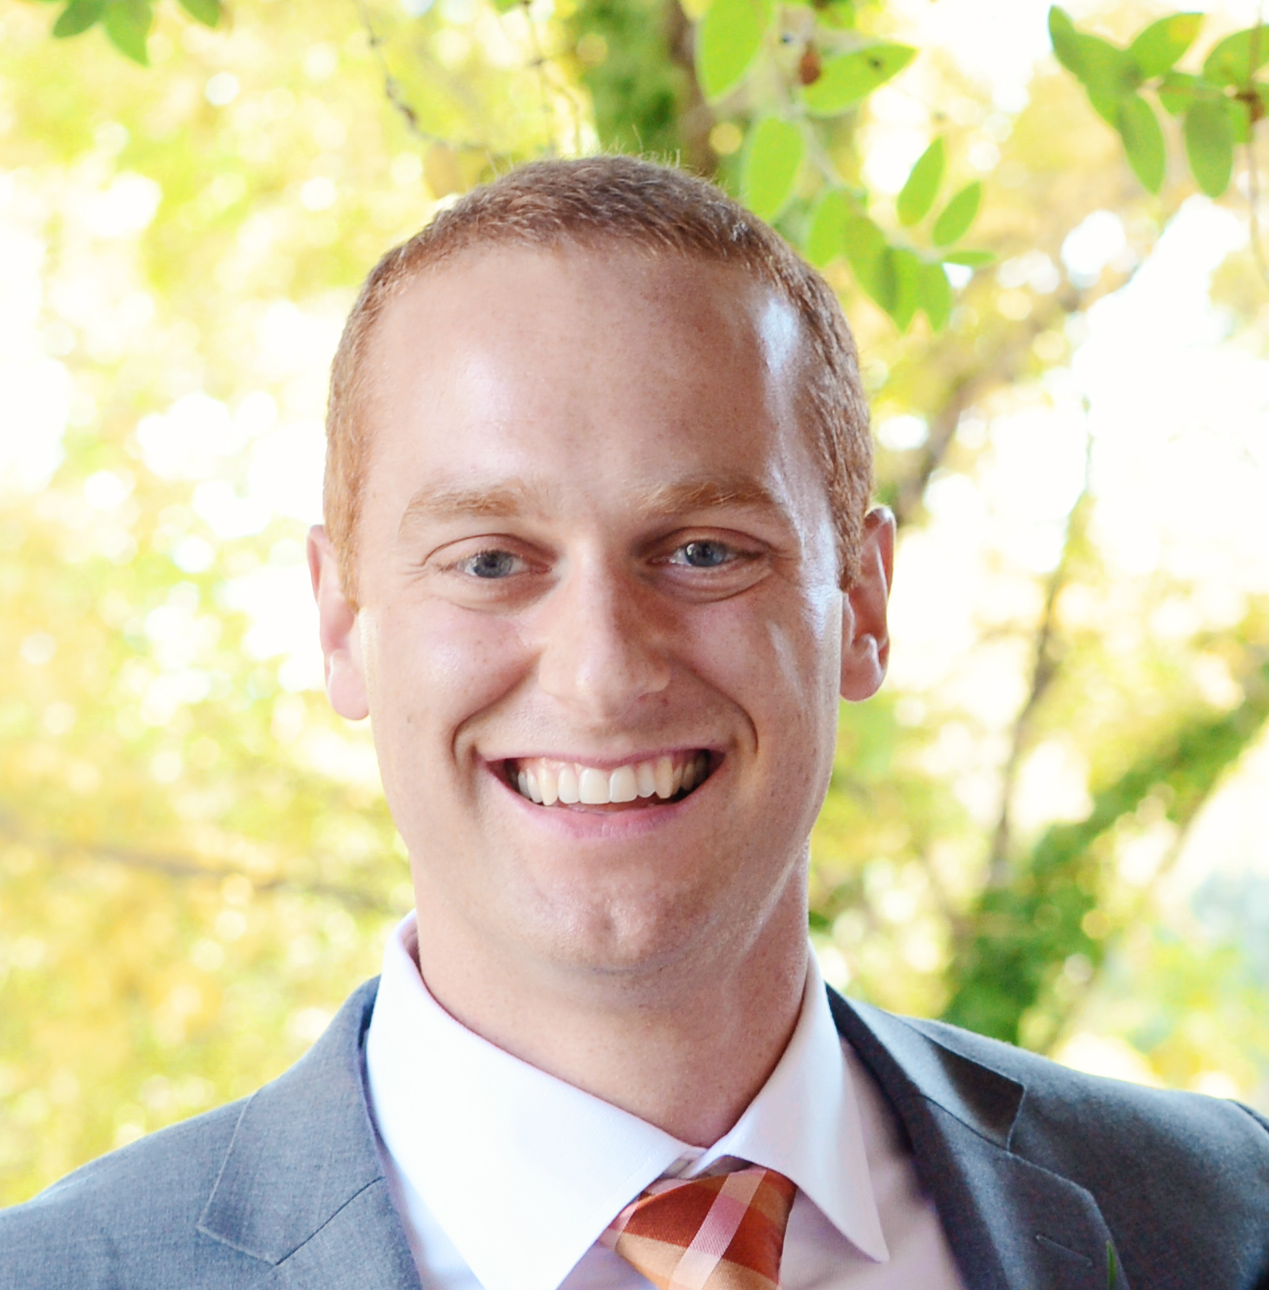
\includegraphics[width=6.5cm,keepaspectratio]{Part I/figures/dpkouri_new.png}
\caption{Drew P. Kouri, Sandia National Laboratories}
\end{figure}
\end{frame}

%%%%%%%%%%%%%%%%%%%%%%%%%%%%%%%%%%%%%%%%%%%%%%%%%
\begin{frame}\frametitle{}
\begin{center}\Large
Section 1: \\
Review and Introduction
\end{center}
\end{frame}
%%%%%%%%%%%%%%%%%%%%%%%%%%%%%%%%%%%%%%%%%%%%%%%%%

%%%%%%%%%%%%%%%%%%%%%%%%%%%%%%%%%%%%%%%%%%%%%%%%%
%%%%%%%%%%%%%%%%%%%%%%%%%%%%%%%%%%%%%%%%%%%%%%%%%
\section{Review and Introduction}
%%%%%%%%%%%%%%%%%%%%%%%%%%%%%%%%%%%%%%%%%%%%%%%%%
%%%%%%%%%%%%%%%%%%%%%%%%%%%%%%%%%%%%%%%%%%%%%%%%%

%%%%%%%%%%%%%%%%%%%%%%%%%%%%%%%%%%%%%%%%%%%%%%%%%
\begin{frame}\frametitle{A Basic Workflow}
\begin{exampleblock}{}
The basic workflow from modeling to numerical solution is as follows.
\begin{itemize}
\item Modeling: PDE, additional constraints, and objective function.

\item Theory: control-to-state map, existence and optimality conditions.

\item Algorithms: function space-based methods (optimize-then-discretize).

\item Numerical Solution: discretize (FD, FEM, wavelets, NN,...) and solve.
\end{itemize}
\end{exampleblock}
\visible<2->{
\begin{exampleblock}{}
Incorporating uncertainty into this workflow adds several new tasks:
\begin{itemize}
\item Modeling: {\color{Red} where/how to include random inputs, model risk preference.}

\item Theory: {\color{Red}  measurability, integrability, \& differentiability: an ``extra step''.}

\item Algorithms: {\color{Red}  sample uncertainty as-you-go versus before-you-go.}

\item Numerical Solution: {\color{Red} when to stop, how to interpret the solution.}
\end{itemize}
\end{exampleblock}
}
\end{frame}
%%%%%%%%%%%%%%%%%%%%%%%%%%%%%%%%%%%%%%%%%%%%%%%%%

%%%%%%%%%%%%%%%%%%%%%%%%%%%%%%%%%%%%%%%%%%%%%%%%%
\begin{frame}\frametitle{}
\begin{center}\Large
Section 1\\
Part I:\\
Modeling: Deterministic and stochastic settings.
\end{center}
\end{frame}
%%%%%%%%%%%%%%%%%%%%%%%%%%%%%%%%%%%%%%%%%%%%%%%%%


%%%%%%%%%%%%%%%%%%%%%%%%%%%%%%%%%%%%%%%%%%%%%%%%%
\subsection{Modeling}
\begin{frame}\frametitle{Choosing the right PDE and Objective}

\begin{example}[Optimization of Optoelectronics]
\centering
      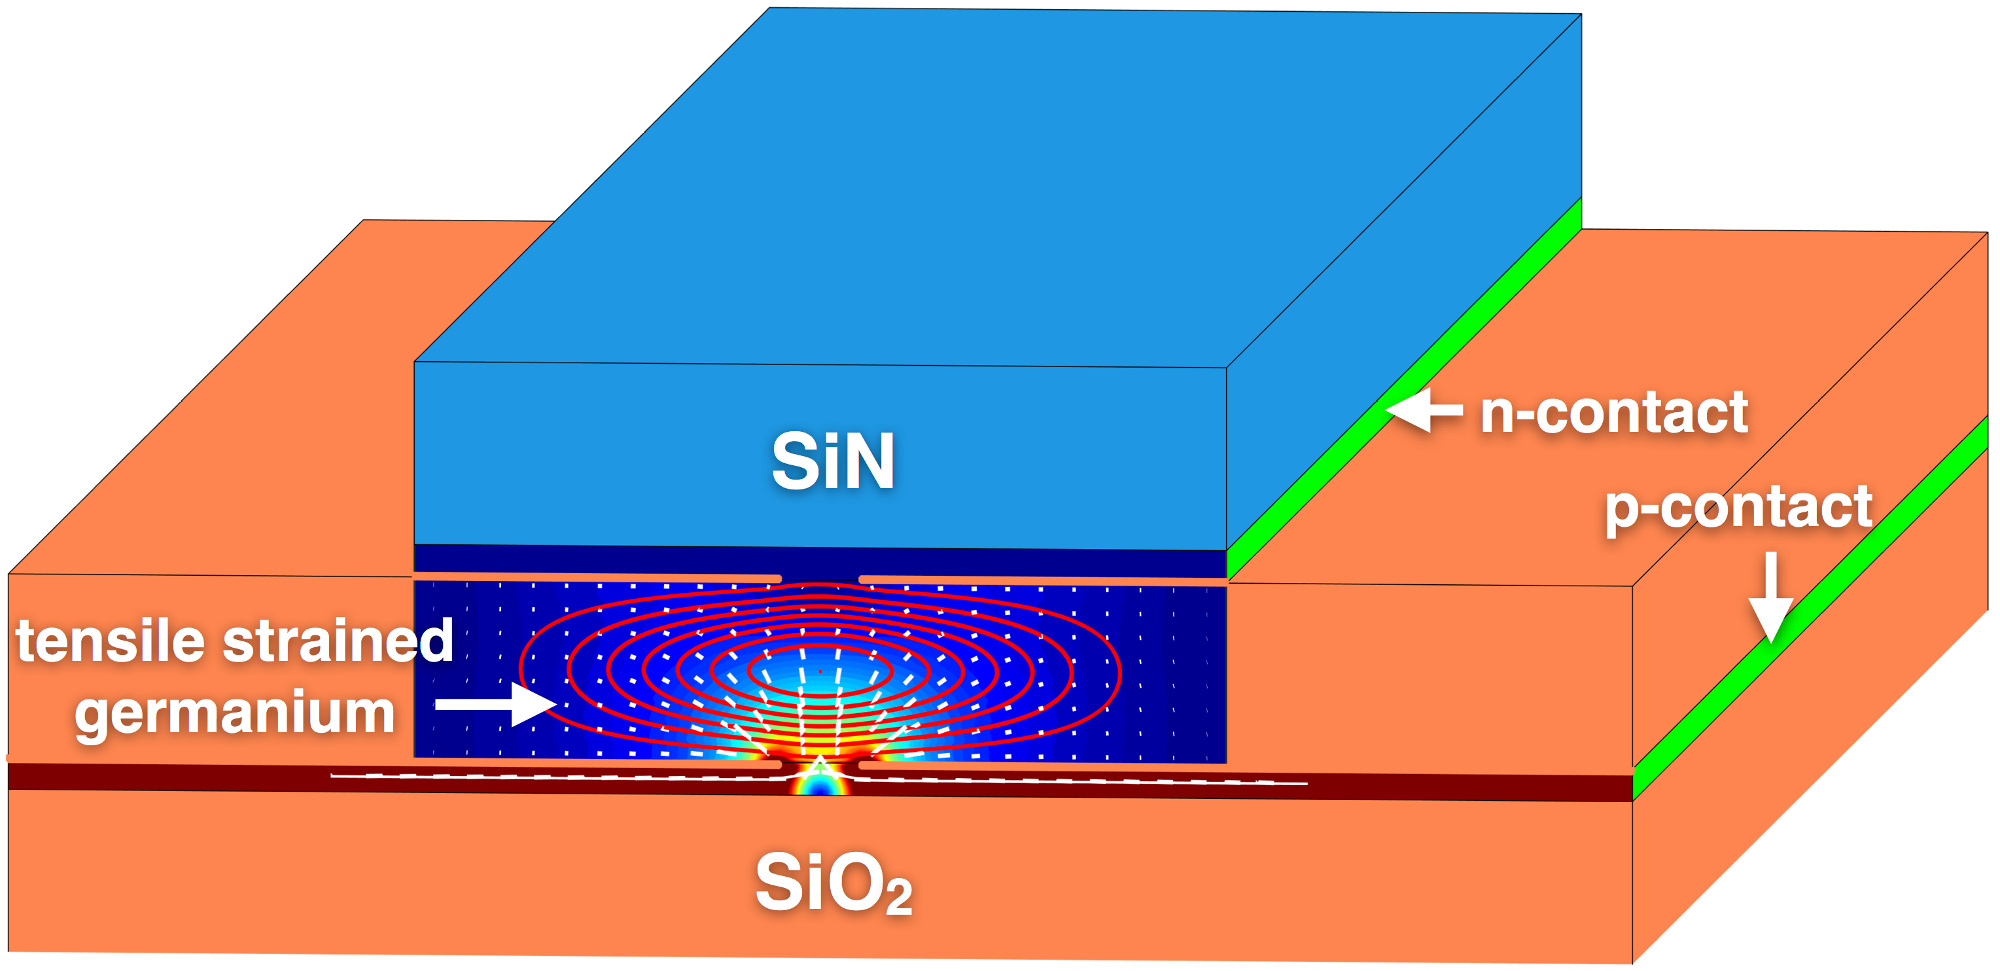
\includegraphics[width=0.6\linewidth]{Part I/figures/graphical_abstract_ieee.jpeg}
\end{example}
\end{frame}

% \begin{frame}\frametitle{Choosing the right PDE and Objective}
% \begin{example}[Optimization of Optoelectronics]
% We need a model that accounts for...
% \begin{itemize}
% \item ...elasticity of the structure (linear elasticity)
% \item ...optical properties (Helmholtz and photon number equation)
% \item ...electronic properties (van Roosbroeck)
% \end{itemize}
% coupled by the layout of the materials Ge, Si, SiN, SiO$_4$, air (decision variables). \medskip
% \visible<2->{
% \begin{columns}[onlytextwidth,T]
% \column{0.6\textwidth}\vspace{1mm}
% The objective function should simultaneously ensure...
% \begin{itemize}
% \item ...tensile strain inside Ge-region is maximized 
% \item ...bulk of support of (at least) first eigenmode
% \end{itemize}
% coincide.
      
% \column{0.4\textwidth}
%   {\centering
%      \vspace{1ex}
%       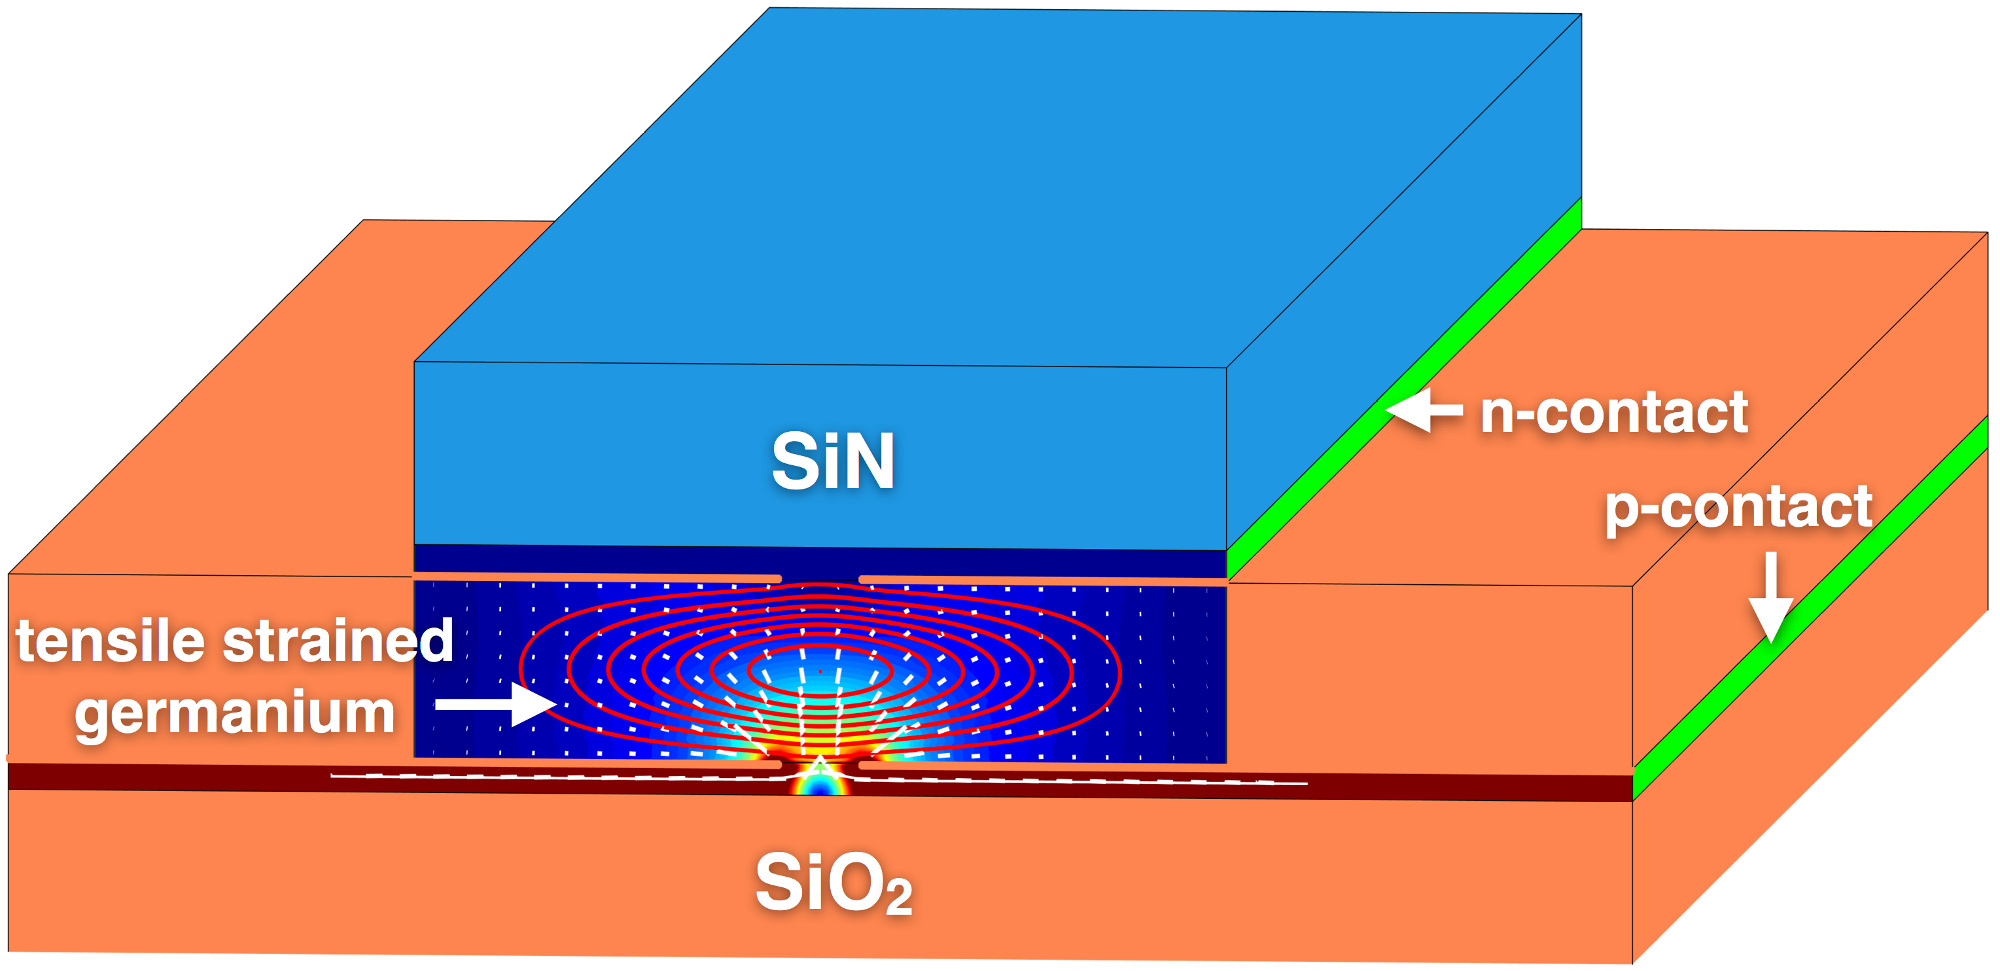
\includegraphics[width=0.7\linewidth]{Part I/figures/graphical_abstract_ieee.jpeg}
%       }
% \end{columns}
% }
% \end{example}
% \end{frame}

% \begin{frame}\frametitle{What is the right PDE model for my application?}
%  \includegraphics[width=\linewidth]{report/pics/schema3.jpg}
% \begin{example}[Optimization of Optoelectronics]
% \begin{itemize}
% \item Theoretically, we know the physical effects of the topology (layout).
% \item What is the simplest effective model?
% \end{itemize}
% \end{example}
%- Show results for just elasticity
%- Show the results for elasticity and Helmholtz
%- Show the gain images from Dirk in our paper
%- Message: It's good to know the ``full'' model, but a simplification might be enough!
%- References: papers with Lukas, Dirk, Michael, Marita's papers.
%- This raises several further points: Even if I know the ``true'' model, do I know all the input parameters? Or have I estimated them from data and inversion approaches? What if I don't fully believe the ``true'' model but I have lots of observations. Can I get away with a simpler model by replacing the inputs with random parameters? 
% \end{frame}

\begin{frame}\frametitle{What is the right PDE?}

\begin{example}[Optimization of Optoelectronics]
\begin{itemize}
\item What is the simplest effective model?
\visible<2->{
\item Optimizing only considering elasticity and first eigenmode yields:}
\end{itemize}
\visible<2->{
\begin{figure}
\centering
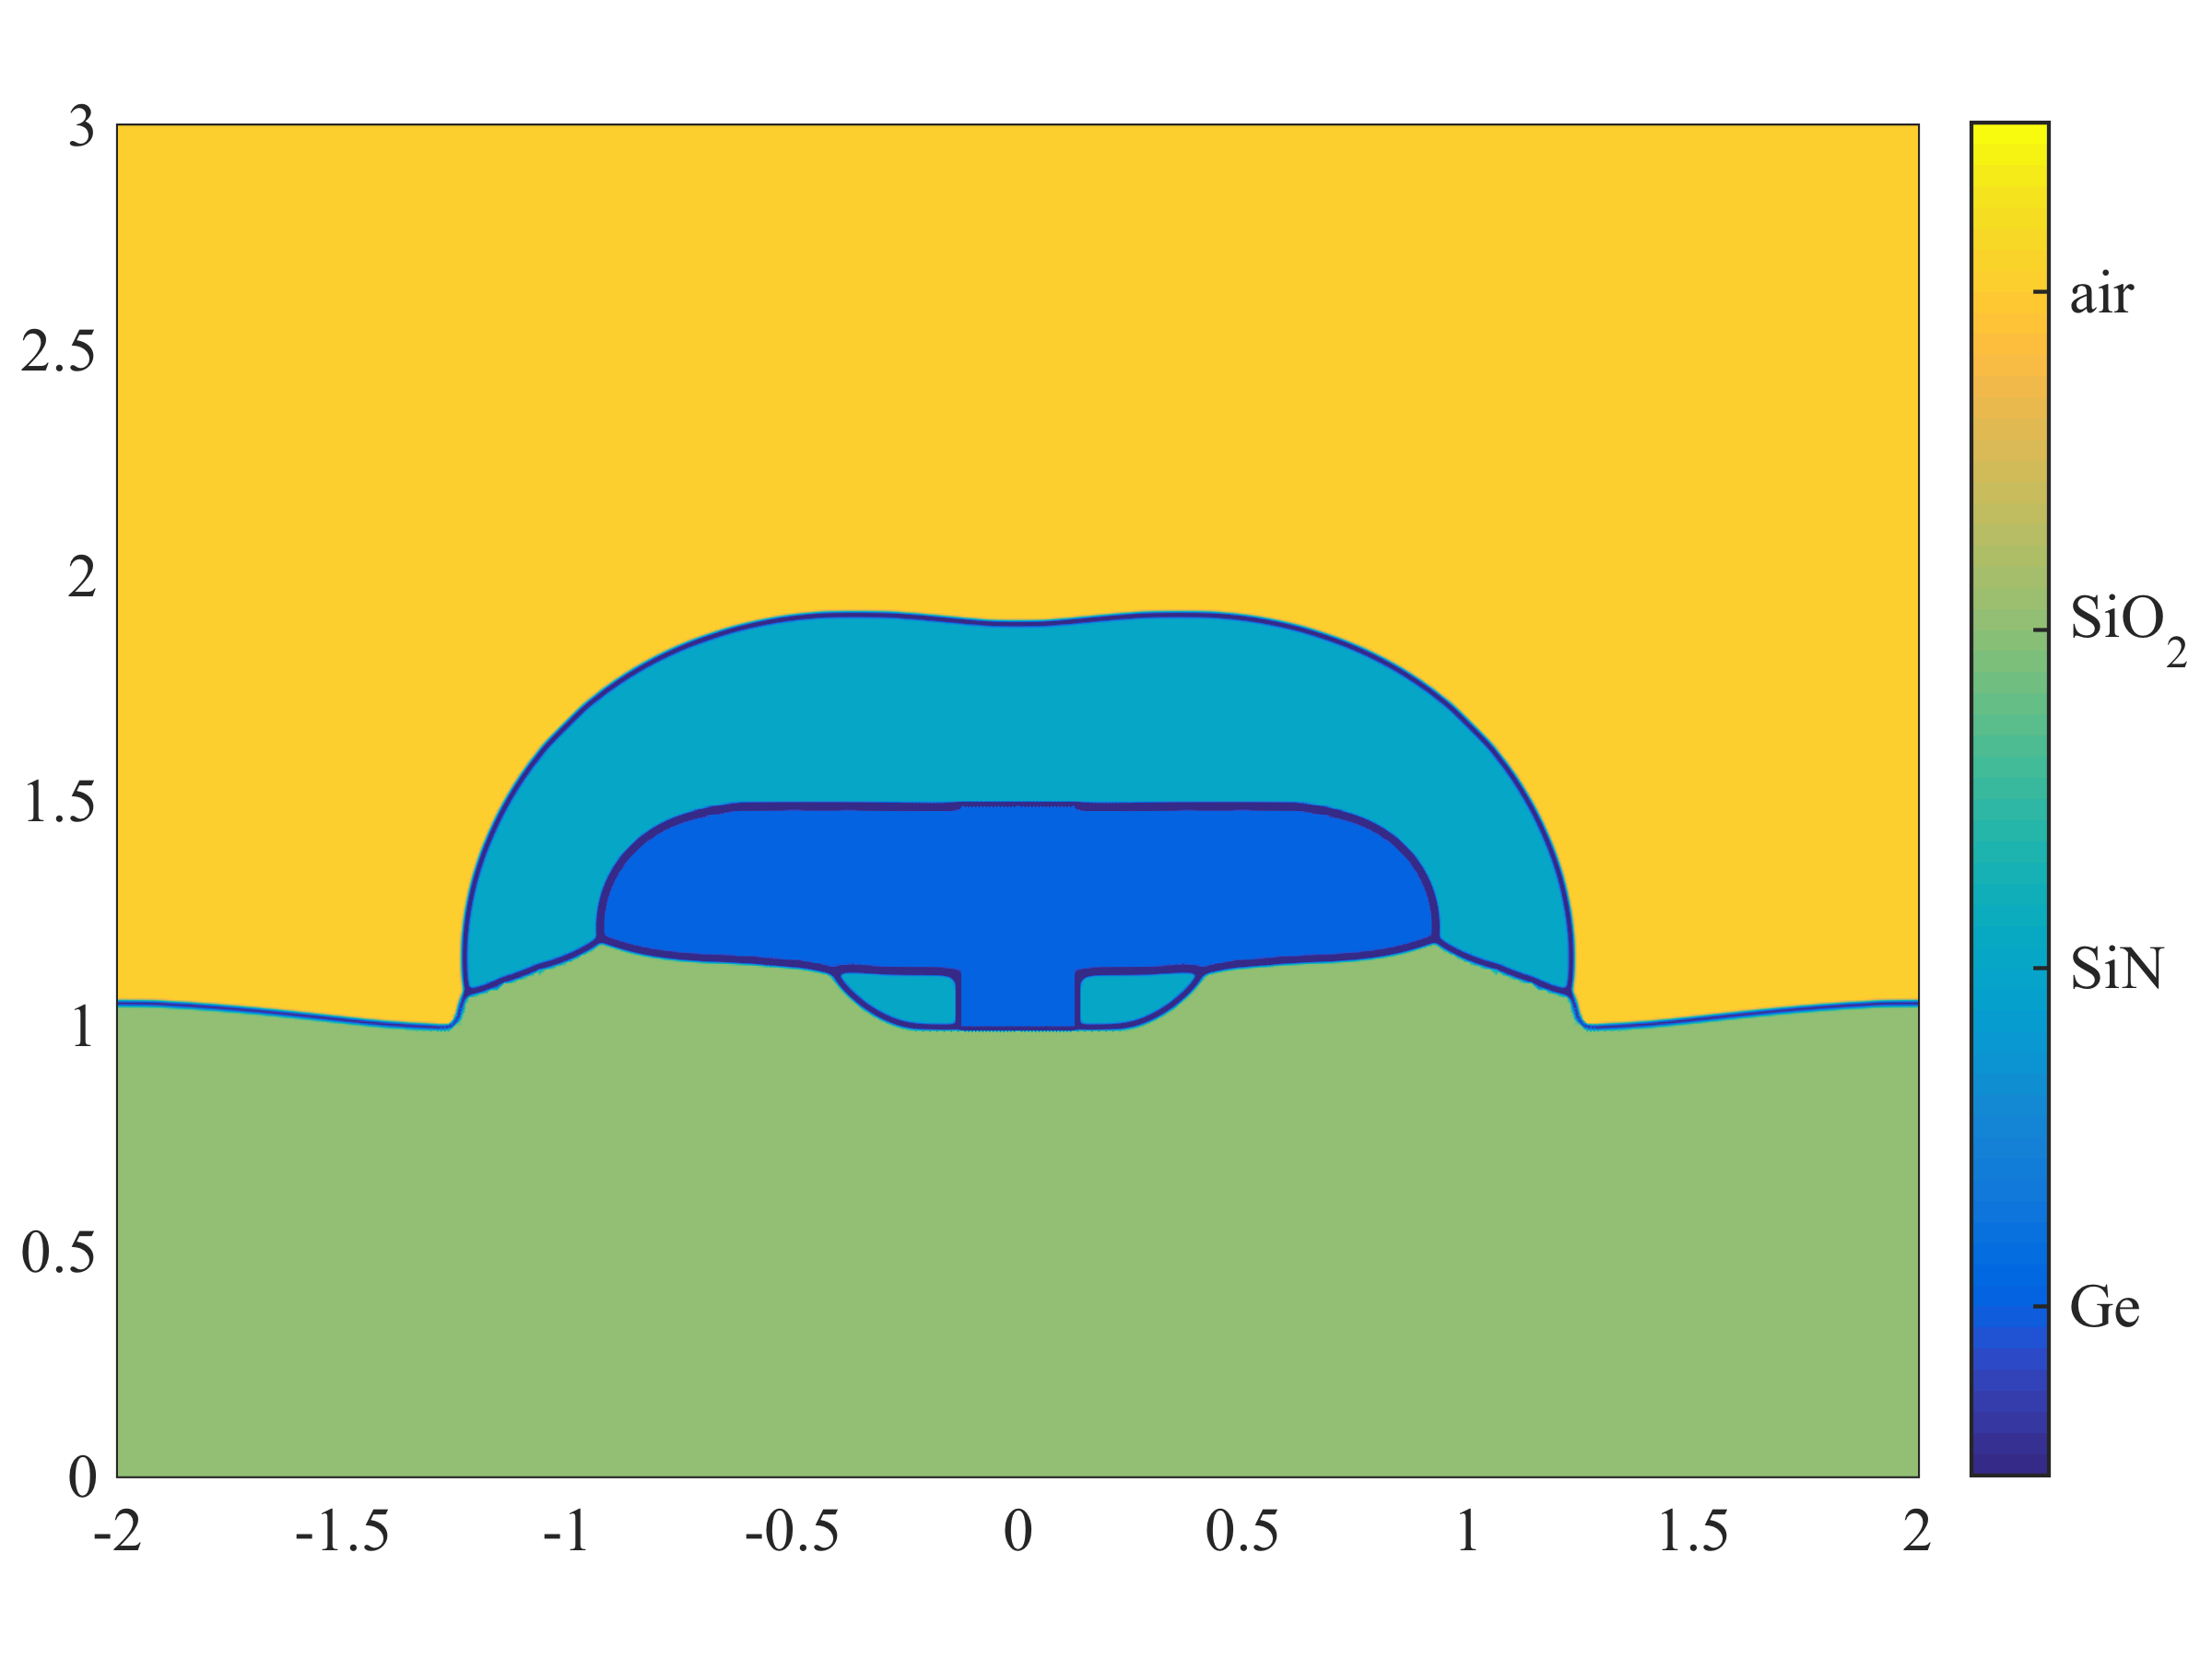
\includegraphics[width=0.3\linewidth]{Part I/figures/topo_FINAL_color.png}
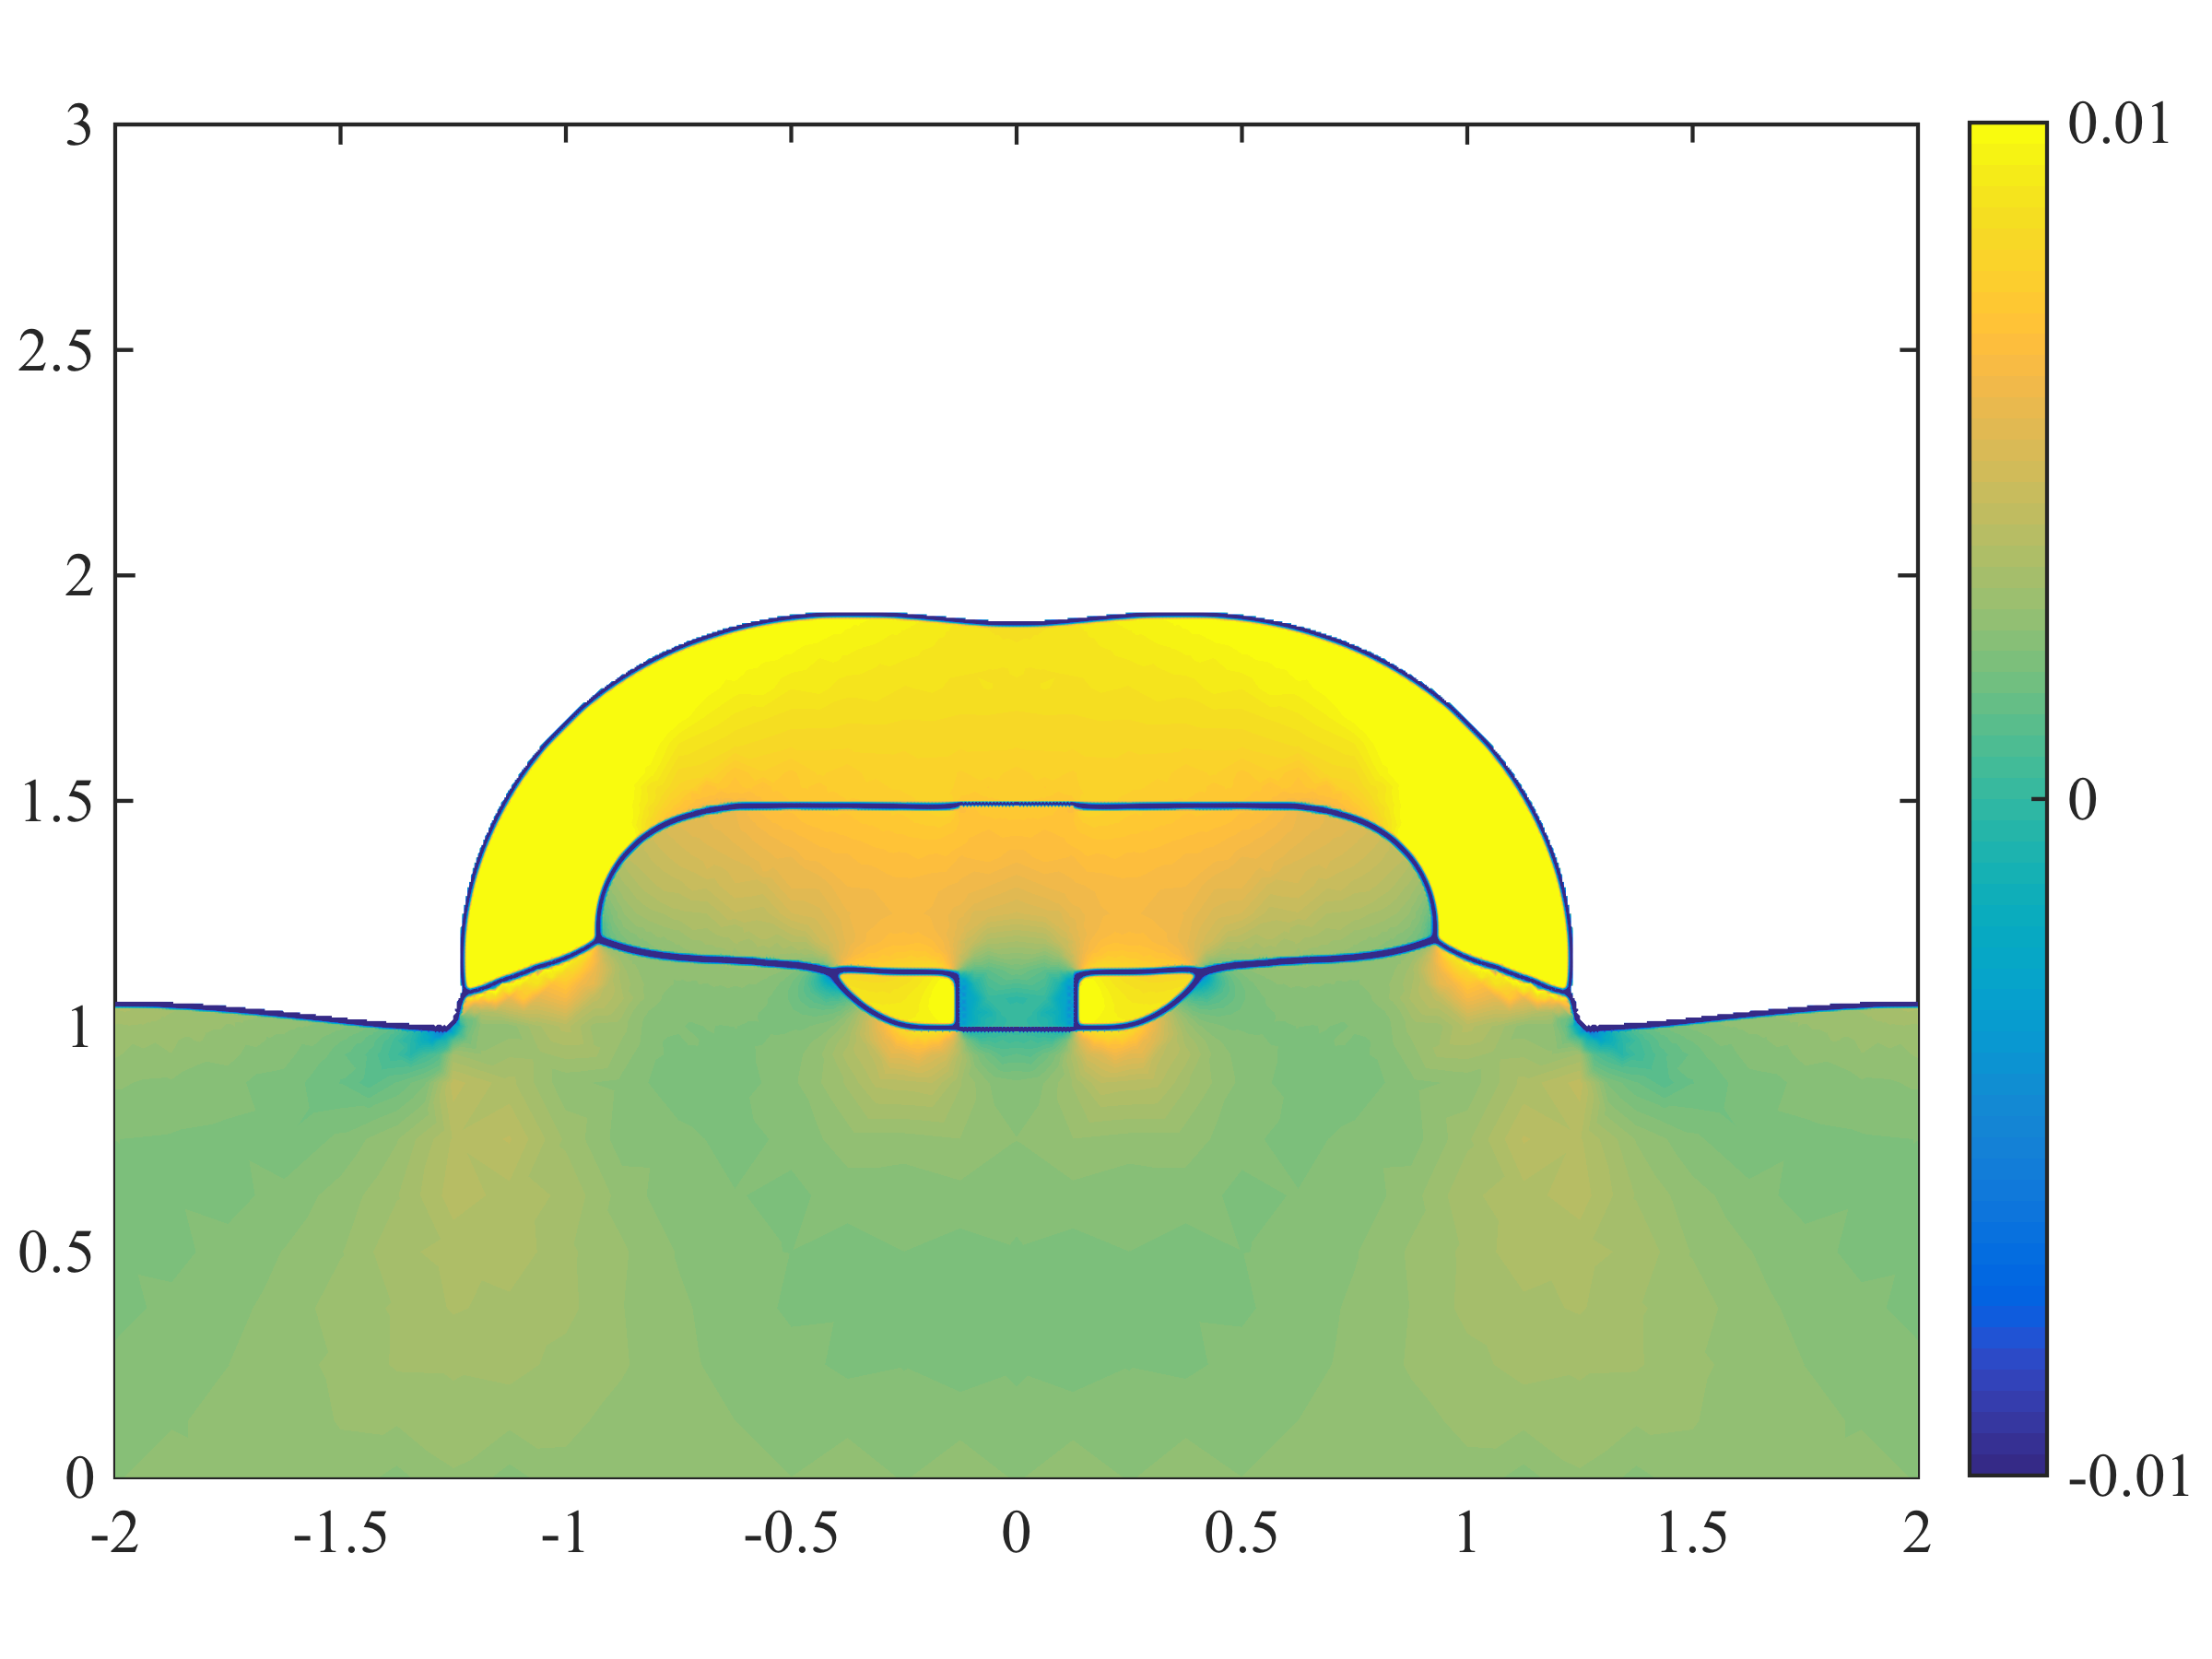
\includegraphics[width=0.3\linewidth]{Part I/figures/strain_FINAL.png}
\caption{\footnotesize Optimal material layout (l.) and its corresponding strain field (r.).}
\label{Figure phi}
\end{figure}
}
\end{example}
\end{frame}

\begin{frame}\frametitle{What is the right PDE?}
\begin{example}[Optimization of Optoelectronics]
\begin{itemize}
\item Simulations of the drift-diffusion system indicate success! 
\end{itemize}
\begin{figure}
\qquad
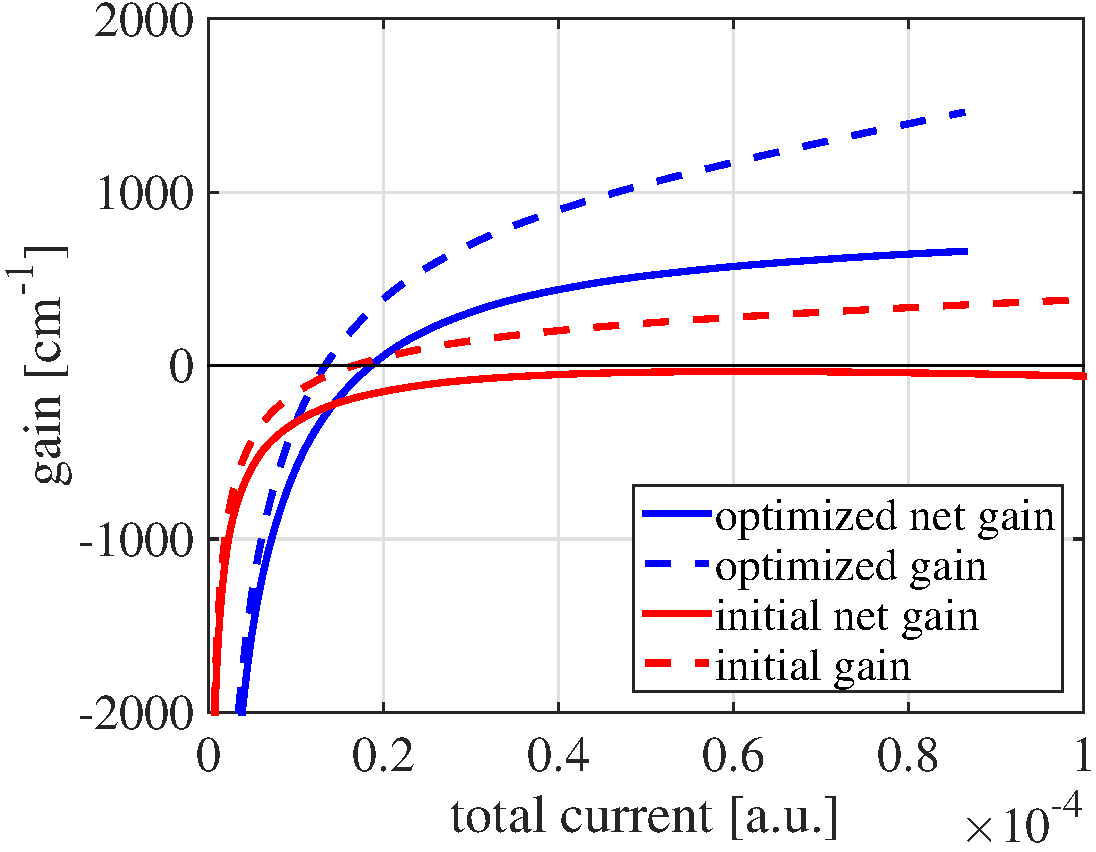
\includegraphics[height=0.24\textwidth, width=0.6\textwidth, keepaspectratio]{Part I/figures/gain-1.pdf}\qquad
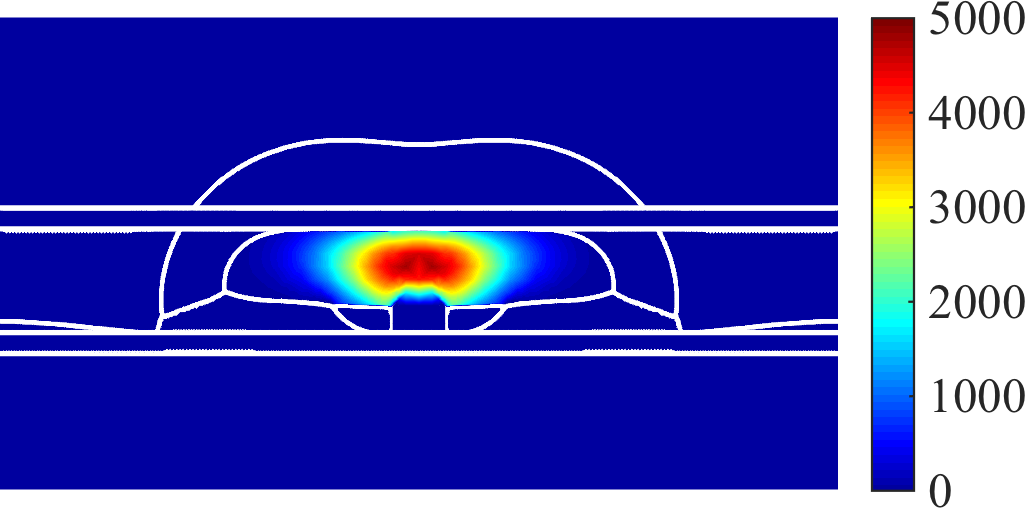
\includegraphics[height=0.24\textwidth, width=0.6\textwidth, keepaspectratio]{Part I/figures/gain_FINAL_new-1.png}%
\caption{
 current-gain characteristics  of initial and optimized device (l.) modal gain $g|\Theta|^2$ [cm$^{-1}$] optimized design (r.)}
\label{fig:gainsimulation}
\end{figure}
\end{example}
\end{frame}

\begin{frame}\frametitle{Do we \alert{really} know the inputs?}
\begin{exampleblock}{}
\begin{minipage}{0.5\textwidth}
    Even if I know the ``true'' model, do I...
\begin{itemize}
\item ...know all the real input parameters?
\item ...have I estimated them from data? 
\end{itemize}
\begin{itemize}
\item What if I don't fully \textbf{trust} the ``true'' model? 
% \item Can I use a simpler model by replacing the inputs with \textbf{random parameters} after \textbf{learning} their distributions from \textbf{data}?
\end{itemize}
\end{minipage}
\begin{minipage}{0.4\textwidth}
    \begin{figure}
        \centering
        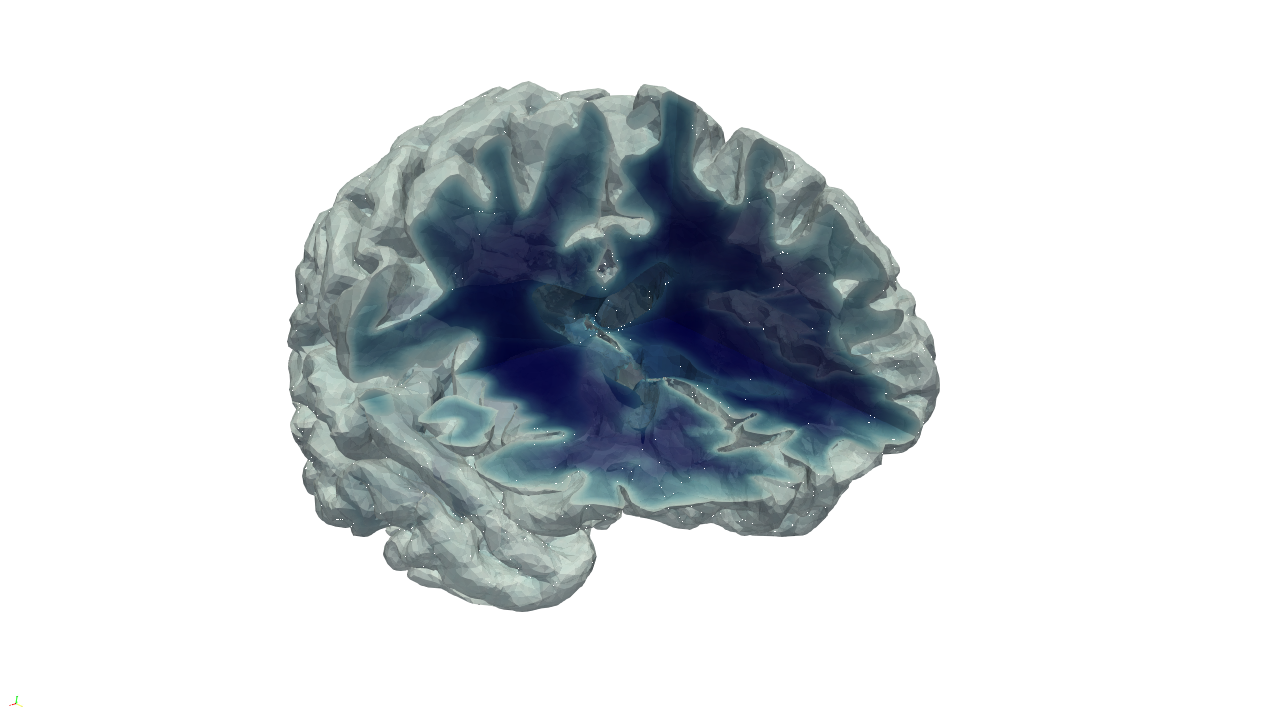
\includegraphics[width=\textwidth,keepaspectratio]{Part I/figures/brain-mesh.png}
         \caption{Tracer concentration estimates (J. Riseth et al \cite{})}
        \label{fig:enter-label}
    \end{figure}
\end{minipage}
\begin{itemize}
\item We don't wish to \alert{quantify uncertainty}, but \alert{make optimal decisions} in the face of uncertainty.
\end{itemize}
\end{exampleblock}

\visible<2->{
\begin{exampleblock}{}
\centering
These thoughts lead to the focus of our course:\\ \textbf{Optimizing PDEs with Random Inputs.}
\end{exampleblock}
}
\end{frame}

\begin{frame}\frametitle{How are my decision spaces restricted?}
% \begin{exampleblock}{}
% \centering 
% Aside from the PDEs, bound constraints present further difficulties.
% \end{exampleblock}


\visible<1->{
\begin{exampleblock}{}
\begin{itemize}
\item Topology optimization: 
$z$ $\sim$ material density (takes values between 0,1), 
$\int_{D} z \ \mathrm{d}x \le \gamma$.
\item State constraint: $T$ max.\ allowable deflection, temperature, current, etc.
\end{itemize}
\end{exampleblock}
}
\visible<2->{
\begin{exampleblock}{}
Domain $D \subset \mathbb R^n$ open, bounded;
$a, b, T : D \to \mathbb R$ $a < b$;
$\Phi : Z \to \mathbb R$, $\gamma \in \mathbb R$.
\begin{itemize}
\item Control constraints: \textbf{decisions} $z : D \to \mathbb R$ must fulfill 
\[
a(x) \le z(x) \le b(x) \text{ for a.e. } x \in D
\quad\quad
\text{ or }
\quad\quad
\Phi(z) \le \gamma.
\]
\vspace{-4ex}
\visible<3->{
\item State constraints: \textbf{solutions} $u$ of PDE $u : D \to \mathbb R$ must fulfill 
\[
u(x) \le T \text{ for a.e. } x \in D.
\]
\item Existence, uniqueness of Lagrange multipliers \alert{not guaranteed}.
\item Sometimes the multipliers are only \alert{signed measures} $\mu : \mathcal{P}(D) \to [0,\infty]$.
}
\end{itemize}
\end{exampleblock}
}
\end{frame}

\begin{frame}\frametitle{How are my decision spaces restricted?}
\begin{exampleblock}{}
After incorporating uncertainty:
\begin{itemize}
\item The decision/design/control $z : D \to \mathbb R$ is made \textbf{before the realization of of uncertainty}.
\item The state is a \textbf{random element} $u : (\Omega,\mathcal{F},\mathbb P) \to X(D)$; $X(D)$ function space over $D$.
\visible<2->{
\item If we consider a time-dependent decision-making process, then $z_t : D \to \mathbb R$ may become uncertain. Think: feedback control.}
\visible<3->{
\item State constraints in a random setting can be very challenging: See Caroline Geiersbach's presentation!
}
\end{itemize}
\end{exampleblock}
% \visible<3->{
% \begin{center}
%     \begin{minipage}{0.25\textwidth}
% 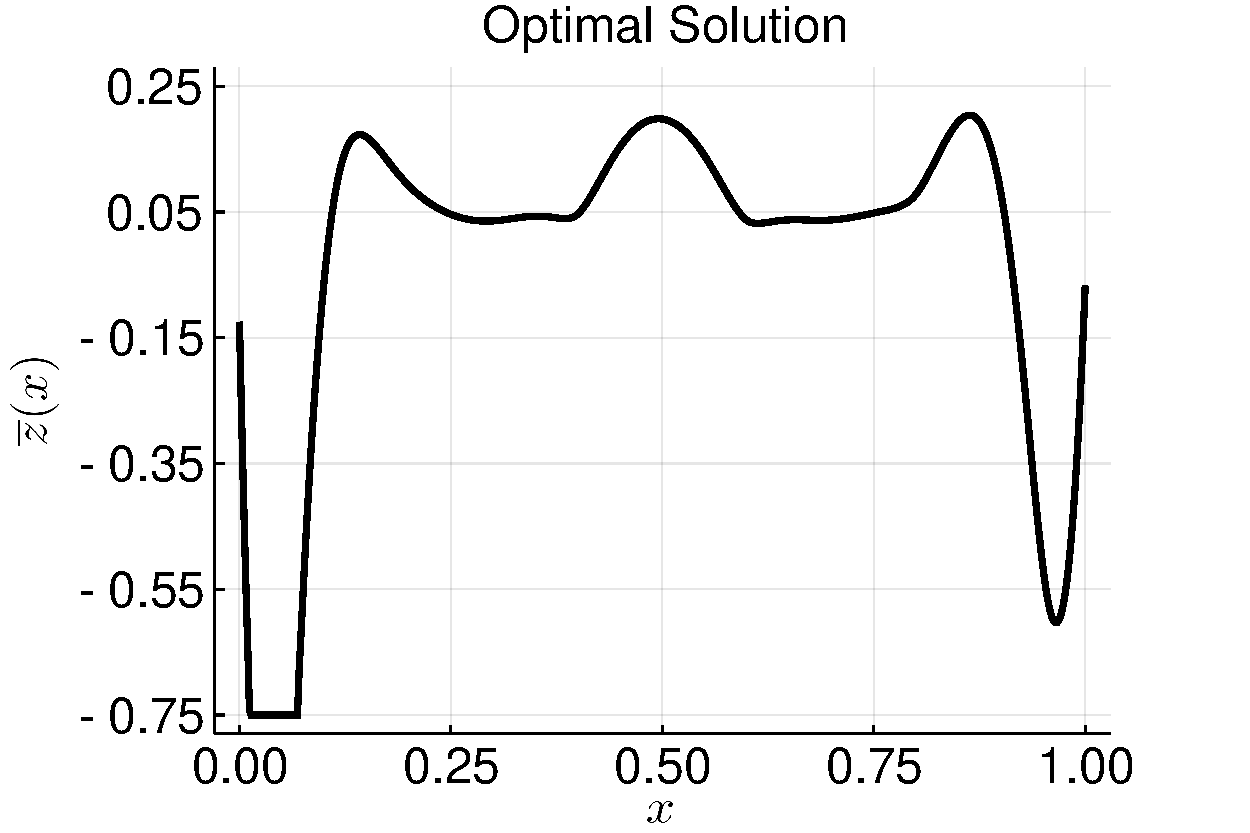
\includegraphics[width=\linewidth]{figures/z_my_1000.pdf}
% \end{minipage}
% \begin{minipage}{0.25\textwidth}
% \includegraphics[width=\linewidth]{figures/oos_my_g1000_M2000.pdf}
% \end{minipage}
% \end{center}
% \begin{figure}
%      \centering
%      \begin{subfigure}[b]{0.5\linewidth}
%          \centering
% %         \includegraphics[width=\textwidth]{graph3}
%           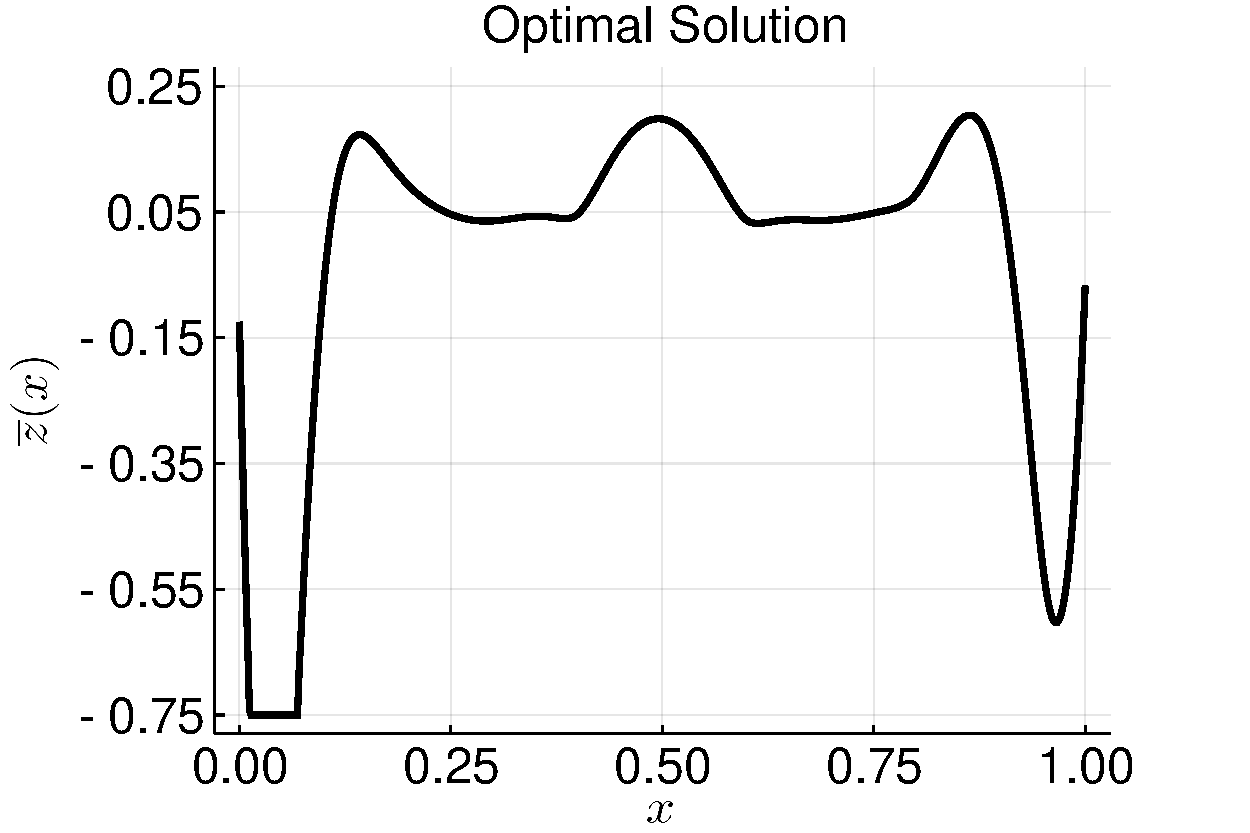
\includegraphics[width=\linewidth]{figures/z_my_1000.pdf}
%          \caption{}
%          \label{fig:opt-ctrl}
%      \end{subfigure}
%      \begin{subfigure}[b]{0.5\linewidth}
%      \centering
%      \includegraphics[width=\linewidth]{figures/oos_my_g1000_M2000.pdf}
%      \caption{}
%      \label{fig:oos-states}
%  	\end{subfigure}
%   \caption{}
%   %       \caption{ (a) Optimal solution $\overline{z}$. (b) Controlled states using $\overline{z}$ for 2000 out of sample instances of $\bm\xi$.
%   % 2.3 \% of cases violate the bound.}
%         \label{fig:saa-ssn}
% \end{figure}
% }

\end{frame}

\begin{frame}\frametitle{Choosing an Objective}

% \only<1>{
% \begin{example}[Optimization of Optoelectronics]
% \begin{itemize}
% \item  \bm $\varphi \sim$ layout of materials, $\bm u \sim$ material displacement, $\Theta \sim$ first eigenmode.
% \item $\int_\Omega j(\bm\varphi,\Theta) \mathrm{tr} e(\bm u) \ \mathrm{d}x \sim$ force overlap of Ge, high tensile strain, $\mathrm{supp}\,\Theta$ 
% \item $\alpha f_{\rm GL}(\bm\varphi,\varepsilon) \sim$ regularizes material boundaries
% \item $J(\bm \varphi, \Theta, \bm u) 
% := 
% \int_\Omega j(\bm\varphi,\Theta) \mathrm{tr} e(\bm u) \ \mathrm{d}x
% +
% \alpha f_{\rm GL}(\bm\varphi,\varepsilon)$.
% \end{itemize}
% \end{example}
% }
\only<1>{
\begin{example}[Optimal Control: Tracking-Type Functionals]
\begin{itemize}
\item Minimize distance of $u$ to $u_d$ (desired state) with minimal cost $\alpha > 0$.
\[
J(u,z) := \frac{1}{2} \| u - u_{d} \|^2_{L^2(D)} + \frac{\alpha}{2} \| z \|^2_{L^2(D)}.
\] 
\end{itemize}
\end{example}
}
\only<2>{
\begin{example}[Minimal Compliance in Topology Optimization]
\begin{itemize}
\item Find a material density $z : D \to \mathbb R$ that minimizes compliance 
\[
J(z) := (F, S(z))_{L^2(D)} + (g,S(z))_{L^2(\partial D)}
\]
\item  $F$ fixed force in the bulk; traction forces $g$ on $\Gamma_{N} \subset \partial D$ also possible.
\end{itemize}
\end{example}
}
\end{frame}

\begin{frame}\frametitle{Dealing with random objectives}
\begin{exampleblock}{}
Using \textbf{random PDE}, means our objective becomes \textbf{implicitly random}:
\[
\min_{z \in Z_{\rm ad}} \mathcal{J}(S(z))(\omega) + \rho(z)
\]
\begin{itemize}
\item $z \in Z_{\rm ad}$ decision variables, designs, controls, etc. (\textbf{deterministic})
\item $z \mapsto S(z)$ solution of the random PDE.  (\textbf{stochastic})
\item $\mathcal{J}$ objective. (either \textbf{deterministic} or \textbf{stochastic})
\item $\rho$ cost or regularization term.
\end{itemize}
\end{exampleblock}
% \only<2>{
% \begin{exampleblock}{}
% \centering Since $\mathcal{J}(S(z))(\omega)$ is a random variable, this problem doesn't make sense yet.
% \end{exampleblock}}
% \only<3>{
% \begin{exampleblock}{}
% \centering What does it mean if my objective is a random variable? 
% \end{exampleblock}
% }
% \only<4>{
% \begin{exampleblock}{}
% \centering What can I hope to achieve?
% \end{exampleblock}
% }
\end{frame}

\begin{frame}\frametitle{Understanding OUU. An Example.}
\begin{exampleblock}{}
\begin{itemize}
\item $f(x,\omega) := \frac{1}{2}(\alpha_1(\omega) x_1^2 + \alpha_2(\omega) x_2^2) - (\beta_1(\omega) x_1 + \beta_2(\omega) x_2).$
\item $\alpha_i \sim U(0,1)$, $\beta_i \sim N(0,1)$ for $i=1,2$.
\item The stochastic optimization problem 
$
\min_{x \in \mathbb R^2 } \mathbb E[f(x)]
$
has unique solution $(x^{\star}_1,x^{\star}_2) = (0,0)$. 
\item $f(x^{\star},\cdot)$ is a degenerate r.v.: $\mathbb P(\left\{\omega \in \Omega \; \left| f(x^{\star},\omega) = 0\right.\right\}) = 1$
\end{itemize}
\begin{center}
    \begin{minipage}{0.6\textwidth}
        Solving iteratively, the sample cdf's converge:
    \end{minipage}
    \begin{minipage}{5cm}
        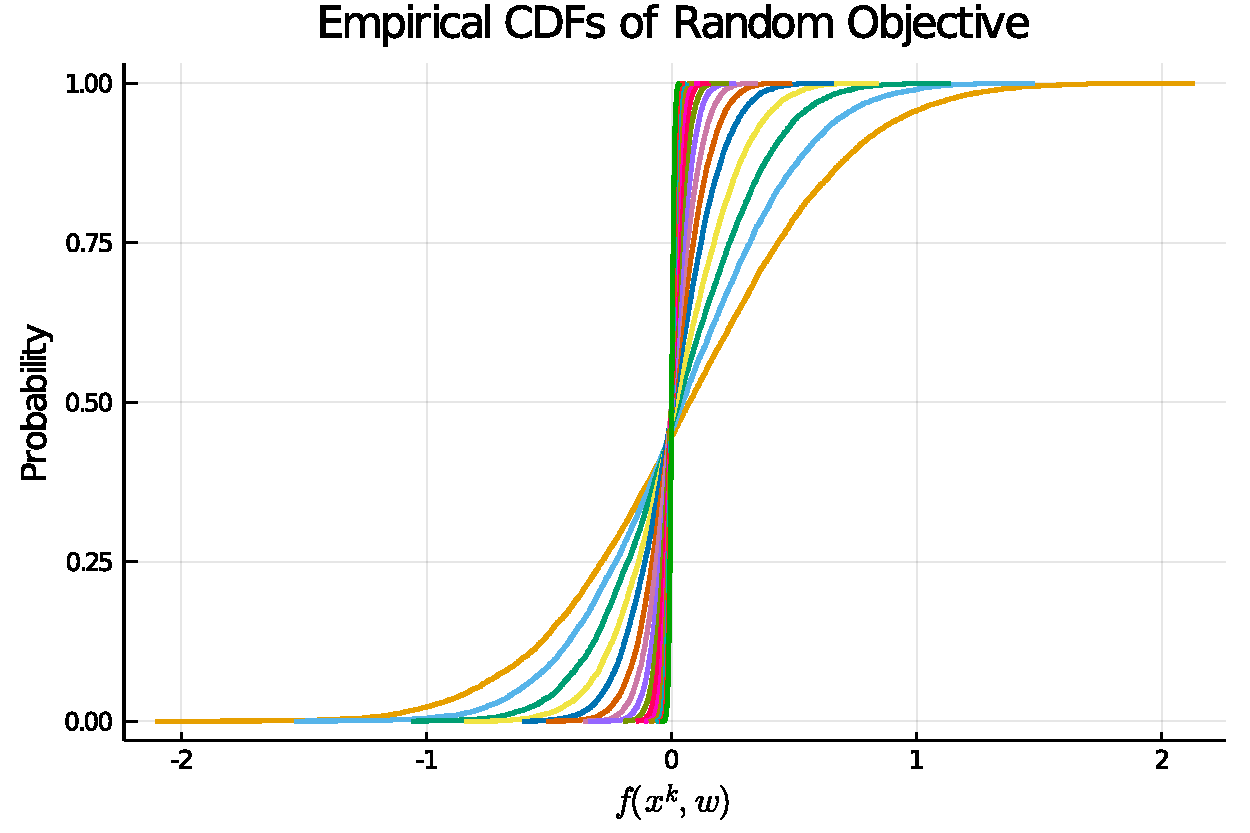
\includegraphics[width=\textwidth, keepaspectratio]{Part I/figures/empirical_cdfs_obj.pdf}
    \end{minipage}
\end{center}

\end{exampleblock}
\end{frame}

\begin{frame}\frametitle{Shaping the Distribution}
\begin{exampleblock}{}
\begin{itemize}
% \item This is an extreme example. 
\item We choose a \textbf{numerical surrogate for risk} that \textbf{shapes the distribution} of
\[
X_{z^{\star}}(\omega) := \mathcal{J}(S(z^{\star}))(\omega) + \rho(z^{\star}).
\] 
\item E.g., if $X_{z} \ge a$ for all $z \in \Zad$, then  $|F_{X_{z^{\star}}}^{-1}(0.95)-a|$ should be small.
\item $F_{X_{z^{\star}}}^{-1}(0.95)$ is the upper 95\% quantile of $X_{z^{\star}}$.
\[
F_{X_{z^{\star}}}^{-1}(0.95) := \inf \{ \alpha : \mathbb P(X_{z^{\star}} \le \alpha ) \ge 0.95 \}
\]
\end{itemize}
\end{exampleblock}
\begin{exampleblock}{}
\centering
For now, we will consider the objectives $\risk[\mathcal{J}(S(z))]$ and specify $\risk$ later.
\end{exampleblock}
\end{frame}
%%%%%%%%%%%%%%%%%%%%%%%%%%%%%%%%%%%%%%%%%%%%%%%%%

\begin{frame}\frametitle{}
\begin{center}\Large
Section 1\\
Part II:\\
Examples: Making the discussion concrete.
\end{center}
\end{frame}

%%%%%%%%%%%%%%%%%%%%%%%%%%%%%%%%%%%%%%%%%%%%%%%%%
\subsection{Examples}

\begin{frame}\frametitle{Ex: A Contaminant Mitigation Problem}
\begin{exampleblock}{}
\smaller
Find optimal placement of mitigating factors $z$ by solving:
\begin{equation*}\label{eq:optprob_ex2}
  \min_{z\in\Zad}\left\{
    {\color{blue}\risk}\left[\frac{\kappa_s}{2}\int_{D} S(z)^2\,\mathrm{d}x\right]
       + \kappa_c \|z\|_1\right\}
\end{equation*}
where
 $\kappa_s = 10^5$, $\kappa_c =1$ and $S(z) = u:\Omega\to H^1(D)$ solves
the weak form of
\begin{align*}
  -\nabla\cdot(\alert{\epsilon(\omega)}\nabla u) + \alert{\mathbb{V}(\omega)}\cdot\nabla u
    &= \alert{f(\omega)} - Bz &\quad\text{in $D$, a.s.}\\
  u &=0 &\quad \text{on $\Gamma_d = \{0\}\times(0,1)$, a.s.} \\
 \alert{ \epsilon(\omega)}\nabla u\cdot n &= 0 &\quad\text{on $\partial D\setminus\Gamma_d$, a.s.}
\end{align*}
\begin{itemize}\vspace*{-3ex}
\item $D = (0,1)^2$ is the physical domain, $(\Omega,\mathcal{F}, \bbp)$ complete probability space
\item $\mathcal{Z}$ is the control space, e.g., $L^2(D)$ or $\mathbb R^n$; $\Zad = \{z\in \mathcal{Z}\,\vert\,0\le z\le 1\}$.
\item $u$ is the advected pollutant.
\item $\risk : \mathcal{X} \to \overline{\mathbb R}$ is a numerical surrogate for ``risk'', i.e., a risk measure.
\end{itemize}
Random inputs: $\alert{\epsilon, \mathbb V, f}$ permeability, wind, sources of contaminant.
\end{exampleblock}
\end{frame}

\begin{frame}\frametitle{Ex: Topology Optimization}

\begin{exampleblock}{}
\smaller
Find an optimal material distribution $z^{\star}$ that minimizes compliance by solving
      \[
      \min_{z \in \Zad}\;
         {\color{blue}\risk}\left[
            \int_D \alert{F(\cdot)}\cdot S(z)\,\mathrm{d}x\right] + \wp(z)
      \]
      where $S(z)=u$ solves \vspace{-1ex}
      \begin{align*}
        -\nabla\cdot(\alert{\mathbf{E}(\omega)}(z):\epsilon u)
            =&\; \alert{F(\omega)} &&\text{in }D\textcolor{white}{.} \\
        \epsilon u =&\;
           \tfrac{1}{2}(\nabla u + \nabla u^\top)
           &&\text{in }D\textcolor{white}{.}\\
         u =&\; \alert{g}(\omega) &&\text{on }\partial D
      \end{align*}
and the material density $z \in \Zad$ fulfills 
\begin{itemize}
\item $z : D \to \mathbb R$.
\item $z(x) \in [0,1]$ a.e.\ on $D$ ($z = 0$ ``no material'', $z = 1$ ``material'').
\item  $\int_D z\,\mathrm{d}x \le V_{\textup{\tiny 0}}|D|$ (volume fraction).
\end{itemize}
 
Random inputs: Linear elastic isotropic material with \alert{uncertain}
Lam\'e coefficients $\alert{\mathbf{E}}$
traction forces $\alert{g}$ 
 bulk forces $\alert{F}$.

\end{exampleblock}
\end{frame}

% \begin{frame}\frametitle{Ex: Chemical Vapor Deposition}
% \begin{exampleblock}{}
% \smaller
% \begin{minipage}{0.29\textwidth}
%   \centering
%     \begin{tikzpicture}[scale=2.2]
%       \node[inner sep=0pt] (result) at (0.5,0.5)
%         {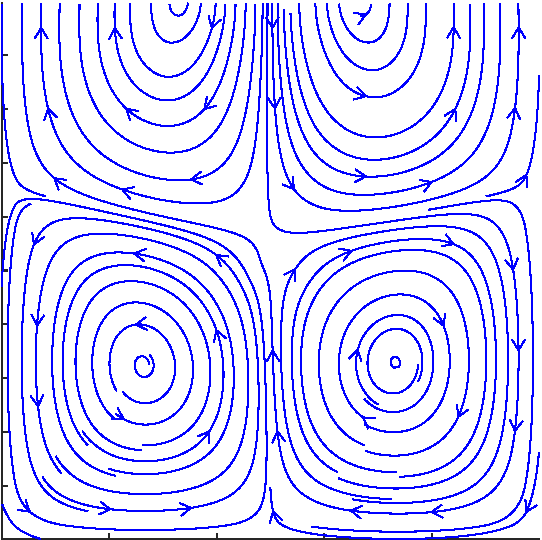
\includegraphics[width=0.72\textwidth]{Part I/figures/mean_uncontrolled_velocity_vort.pdf}};
%       \draw[line width=1pt] (0,0) rectangle (1,1) node[pos=0.5] {$D$};
%       \draw[line width=1pt, blue] (0,1) parabola bend (1/6,19/18) (1/3,1);
%       \draw[line width=1pt, blue] (1/3,1) parabola bend (1/2,8/9) (2/3,1) node[above, xshift=-0.4cm] {In/Outflow};
%       \draw[line width=1pt, blue] (2/3,1) parabola bend (5/6,19/18) (1,1);
%       \draw[line width=1.5pt, red] (0,0) -- (1,0) node[below left, xshift=-0.3cm] {Substrate};
%       \draw[line width=1.5pt, black!70!green] (0,0) -- (0,1) node[left, xshift=-0.3cm, yshift=-0.5cm, rotate=90] {Control};
%       \draw[line width=1.5pt, black!70!green] (1,0) -- (1,1) node[right, xshift=0.3cm, yshift=-0.5cm, rotate=-90] {Control};
%     \end{tikzpicture}
% \end{minipage}\hfill
% \begin{minipage}{0.65\textwidth}\vspace{-3mm}
% \[
%   \min_{z\in\Zad}\; \frac{1}{2}{\color{blue}\risk}\left[\int_{D} (\nabla\times V(z))
%     \,\mathrm{d}x\right] + \frac{\gamma}{2}\int_{\Gamma_c} |z|^2 \,\mathrm{d}x
% \]
% where $(V(z),P(z),T(z)) = (v,p,\tau)$ solves  \vspace{-1ex}
% \begin{align*}
%   -\alert{\nu(\omega)}\nabla^2 v + (v\cdot\nabla)v + \nabla p
%       + \alert{\eta(\omega)} \tau g &= 0
%     && \text{in }D \\
%  %\nabla \cdot v &= 0 &&\text{in }D\\
%   -\alert{\kappa(\omega)} \Delta \tau + v\cdot\nabla \tau &= 0
%     && \text{in }D\\
%   \alert{\kappa(\omega)} \nabla \tau\cdot n + \alert{h(\omega)}(z-\tau) &=0
%     && \text{on }\Gamma_c
% \end{align*}
% \end{minipage}
% \begin{itemize}
% \item Find an equilibrium boundary temperature $z : \Gamma_c \to \mathbb R$ that minimizes the vorticity in CVD reactor.
% \item $V$ velocity, $P$ pressure, $T$ temperature.
% \item Possible random inputs:  kinematic viscosity $\alert{\nu}$, thermal expansion coefficient  $\alert{\eta}$, thermal conductivity $\alert{\kappa}$,  heat transfer coefficient due to rugosity $\alert{h}$. 
% \end{itemize}
% \end{exampleblock}
% \end{frame}

%%%%%%%%%%%%%%%%%%%%%%%%%%%%%%%%%%%%%%%%%%%%%%%%%
\subsection{Theory}

\begin{frame}\frametitle{}
\begin{center}\Large
Section 1\\
Part III:\\
Theory: How to handle PDE-constraints
\end{center}
\end{frame}


\begin{frame}\frametitle{PDE-constraints}
\visible<1->{
\begin{exampleblock}{}
A PDE-constraint can be viewed as requiring
\[
\vspace{-1ex}
e(u,z) = 0,
\vspace{-1ex}
\]
where
\begin{itemize}
\item  $e : U \times Z \to W$
\item $U$ is the \textbf{state space}, $Z$ is the \textbf{control space}, $W$ is typically the dual space $U^*$.
\end{itemize}
\end{exampleblock}
}
\visible<2->{
\begin{exampleblock}{}
\begin{itemize}
\item The ``\textbf{reduced space approach}.''
\item  There exists a continuous, differentiable mapping $z \mapsto S(z)$ such that 
\[
e(S(z),z) = 0,
\]
so the PDE can be treated implicitly.  
\item $S$ is often called the ``\textbf{control-to-state mapping.}'' 
\end{itemize}
\end{exampleblock}
}
\end{frame}

\begin{frame}\frametitle{What do I know about the PDE?}
\begin{exampleblock}{}
\begin{itemize}
\item $D \subset \mathbb R^n$ open, bounded set with Lipschitz boundary $\Gamma$.
\item $f \in L^2(D)$, $g \in H^{-1/2}(\Gamma)$, $u_0 \in H^1(\Gamma)$, $\eta > 0$.
\end{itemize}
\end{exampleblock}
\only<2>{
\begin{exampleblock}{Linear Elliptic Boundary Value Problem}
There exists a \textbf{unique solution} $u \in H^1(D)$ that solves the weak form of 
\[
\aligned
-\Delta u + u        &= f \text{ in } D&\\
\partial_{\bm n} u &= g \text{ on } \Gamma&
\endaligned
\]
The mapping $(g,f) \mapsto u$ is \textbf{bounded and linear} $\Longrightarrow$ $S(z)$ continuous, differentiable.
\end{exampleblock}}
\only<3>{
\begin{exampleblock}{Nonlinear Boundary Value Problem (Allen-Cahn)}
There exist \textbf{solution\alert{s}} $u \in H^1(D)$ of 
\[
\aligned
-\Delta u +  u -  u^2 + u^3 &= f \text{ in } D&\\
\partial_{\bm n} u &= \eta(u - u_{0}) \text{ on } \Gamma&
\endaligned
\]
$\Longrightarrow$ $S(z)$ is \alert{set-valued}.
\end{exampleblock}
}
\end{frame}

\begin{frame}\frametitle{What do I know about the PDE?}
\begin{exampleblock}{}
\begin{itemize}
\item Without single-valued $S(z)$, theory and algorithmic approaches are more difficult. 
\item \visible<2->{
\textbf{Full space approach:} Need derivatives $e_u(u^{\star},z^{\star}), e_y(u^{\star},z^{\star})$ at a solution  $(u^{\star},z^{\star})$ and 
$
e'(u^{\star},z^{\star}) \text{ is surjective }.
$
}
\end{itemize}
\end{exampleblock}
\visible<3->{
\begin{exampleblock}{}
In either case, the workflow becomes 
\begin{itemize}
\item Does there exist a well-defined control-to-state mapping $S(z)$?
\item What regularity does $u$ have? (e.g. $u$ is in $H^1(D)$? $H^2(D)$?)
\item Is $S$ differentiable? What PDE does $w = S'(u) h$ solve?
\end{itemize}
\end{exampleblock}
}
\end{frame}

\begin{frame}\frametitle{Random PDE Constraints}
\begin{exampleblock}{}
Adding random inputs, the constraint can be viewed as 
\[
e(u,z; \omega) = 0\quad \mathbb P\text{-a.s.}.
\]
This adds a few questions to the workflow (assume reduced space approach):
\begin{itemize}
\item Is $u : (\Omega,\mathcal{F}) \to U$ (strongly) \textbf{measurable}? 
\item Is $u : (\Omega, \mathcal{F}) \to U$ \textbf{integrable or essentially bounded}?
\end{itemize}\medskip

Regularity, continuity, etc. now in \textbf{Lebesgue-Bochner spaces} $L^{p}(\Omega, \mathcal{F}, \mathbb P; U)$.
\begin{itemize}
    \visible<2->{
    \item Lebesgue-Bochner spaces used in parabolic PDEs. Time interval $[0,T]$ is replaced by $\Omega$}
    \visible<3->{
    \item $L^{q}(\Omega,\cF,\bbp; U)$ ($q \in [1,\infty)$) (strongly) meas.\ $y : \Omega \to U$:
$
\mathbb E_{\bbp}[ \| y \|^{q}_{U} ] < +\infty.  
$}
    \visible<4->{
    \item $L^{\infty}(\Omega,\cF,\bbp; U)$  ess.\ bounded (strongly) meas.\ $y : \Omega \to U$:
$
\mathrm{ess\, sup}_{\omega \in \Omega}\| y(\omega) \|_{U}  < +\infty.  
$
}
\end{itemize}


\end{exampleblock}
\end{frame}

%\subsection{A Linear Elliptic PDE with Random Inputs}


\begin{frame}\frametitle{A Model Forward Problem}
%(\textbf{Time: 10 min})
\begin{exampleblock}{}
\begin{itemize}
    \visible<1->{
    \item \textbf{Physical Domain:} $D \subset \mathbb R^n$ open bounded subset with Lipschitz boundary $\Gamma \subset \mathbb R^n$. 
    }
    \visible<2->{
    \item \textbf{Inputs:} $A: D \to \mathbb S^{n \times n}$, $f: D \to \mathbb R$ are measurable mappings.
    }
    \visible<3->{
    \item  \textbf{Differential Operator:} $A: D \to \mathbb S^{n\times n}$ induces bounded, uniform elliptic operator.
    }
    \visible<4->{
    \item \textbf{Forcing Term:} $f$ is square-integrable on $D$, i.e., $f \in L^2(D)$.
    }
    \visible<5->{
    \item \textbf{Deterministic Problem:} Find $u: D \to \mathbb R$ such that
\begin{equation}\label{eq:lin_ellip_deter}
\aligned
-\mathrm{div\,}\left(A(x) \nabla u(x) \right) 
&= f(x), &\text{ for } x  &\in D,\\
u(s)
&= 0,          &\text{ for } s &\in \Gamma.
\endaligned
\end{equation}
    }
\end{itemize}\vspace{-2ex}
\end{exampleblock}

\end{frame}

\begin{frame}\frametitle{A Model Forward Problem}
\begin{exampleblock}{}
\begin{itemize}
\visible<1->{
\item For $u \in C^{\infty}_{c}(D)$, define the norm $\| \cdot \|_{U}$ by
\[
\| u \|^2_{U} := \int_{D} \nabla u(x) \cdot \nabla u(x) \, \mathrm{d}x.
\]
\item \textbf{Recall:} Closure of $C^{\infty}_{c}(D)$ w.r.t. $\| \cdot \|_{U}$ is the separable Hilbert space $U := H^1_0(D)$.
}
\visible<2->{
\item For $u, v \in U$, define
\[
a(u,v) := \int_{D} A(x) \nabla u(x) \cdot \nabla v(x) \mathrm{d}x,\quad 
L(v) := \int_{D} f(x) v(x) \mathrm{d}x.
\]
}\vspace{-2ex}
\visible<3->{
\item The \textbf{variational form} of \eqref{eq:lin_ellip_deter}:
Find $u \in U$ such that
\begin{equation}\label{eq:lin_ellip_deter_weak}
a(u,v) = L(v),\quad \forall v \in U.
\end{equation}
\item Lax-Milgram provides existence and uniqueness of $u \in U$.
}
\end{itemize}
\end{exampleblock}
\end{frame}

\begin{frame}\frametitle{A Stochastic Forward Problem}
\begin{exampleblock}{}
\begin{itemize}
\visible<1->{
\item \textbf{Random Domain:} $\Omega$ is a sample space, $\cF \subset \mathcal{P}(\Omega)$ a $\sigma$-algebra, $\bbp : \cF \to [0,1]$ a probability measure
\item $(\Omega, \cF, \bbp)$ is a complete probability space (subsets of null sets are measurable sets).
}
\visible<2->{
\item  \textbf{Random Inputs:} $A: \Omega \to L^{\infty}(D, \mathbb S^{n \times n})$, $f: \Omega \to H^{-1}(D)$ $\cF$-measurable mappings.
}
\visible<3->{
\item \textbf{Parametric Problem:} Find $u: \Omega \to H^1_0(D)$ such that
\begin{equation}\label{eq:lin_ellip_stoch}
\aligned
-\mathrm{div\,}\left(A(\omega,x) \nabla u(\omega,x) \right) 
&= f(\omega,x), &\text{ for } x  &\in D,\\
u(\omega,s)
&= 0,          &\text{ for } s &\in \Gamma.
\endaligned
\end{equation}
holds for all $\omega \in \Omega$.
}
\end{itemize}
\end{exampleblock}
\end{frame}

\begin{frame}\frametitle{A Stochastic Forward Problem}
\begin{exampleblock}{}
\begin{itemize}
\visible<1->{
\item 
 $\mathcal{U} := L^2(\Omega,\cF,\bbp; U)$. Define $a : \cU \times \cU \to \mathbb R$, $L : \cU \to \mathbb R$
\[
\aligned
\mathbf{a}(u,v) 
&= \mathbb E\left[  \int_{D} A(\omega,x) \nabla u(\omega,x) \cdot \nabla v(\omega,x) \mathrm{d}x \right],\quad
\mathbf{L}(v)
=
\mathbb E\left[  \int_{D} f(\omega,x) v(\omega,x) \mathrm{d}x \right].
\endaligned
\] 
}
\visible<2->{
\item \textbf{Variational formulation (random):} Find $u \in \mathcal{U}$ such that
\begin{equation}\label{eq:weak_stoch}
\mathbf{a}(u,v)  = \mathbf{L}(v) \quad \forall v \in \cU.
\end{equation}
\item If $f \in L^2(\Omega,\cF,\mathbb P; U^*)$, and $\mathbf{a}$ is \textbf{$\cU$-coercive}, then there exists a unique solution $u \in \cU$.
\item This is just Lax-Milgram for the Hilbert space $L^2(\Omega,\cF,\mathbb P; U)$.
}
\end{itemize}
\end{exampleblock}
\end{frame}





%\begin{frame}\frametitle{Existence and Sensitivity of Solutions}
%\begin{block}{Data Assumptions}
%\begin{itemize}
%\item In addition to the previous data assumptions concerning boundedness, ellipticity, etc.\ we require:
%$
%f \in \mathcal{L}^{2}(\Omega, \cF, \bbp; U^*);
%$
%and $\exists C, c > 0$:\\
%%\vspace{-4mm}
%\begin{center}
%$|\mathbf{a}(u,v)| \le C \| u \|_{\cU} \| v \|_{\cU}$,\; $\mathbf{a}(u,v) \ge c\| u \|^2_{\cU}$,$\forall u,v \in \cU$.
%\end{center}
%\end{itemize}
%\end{block}
%
%\begin{block}{Details}
%\begin{itemize}
%\item For the latter conditions, suppose $A:\Omega \to L^{\infty}(D)$, $\xi, \zeta \in \mathbb R^n$: \vspace{-2mm}
%\[
%\aligned
%A_{ij}(\omega) \xi_i  \xi_j         &\ge c(\omega) \| \xi \|^2_{\mathbb R^n}\\
%| A_{ij}(\omega) \xi_i \zeta_j | &\le C(\omega) \| \xi \|_{\mathbb R^n} \| \zeta \|_{\mathbb R^n}
%\endaligned
%\]
%for some $C, c \in \mathcal{L}^{\infty}(\Omega, \cF, \bbp)$ : 
%$C \ge c > 0$, $c^{-1} \in \mathcal{L}^{\infty}(\Omega, \cF, \bbp)$.  
%\item Clearly, there exists $\underline{c} \in \mathbb R$ : $c(\omega) \ge \underline{c} > 0$.
%\item
%Then for any $u, v \in \cU$, we have for $\Pae$-$\omega \in \Omega$\vspace{-2mm}
%\[\aligned
% \int_{D} A(\omega,x) \nabla u(\omega,x) \cdot \nabla u(\omega,x) \mathrm{d}x
% &\ge
%  c(\omega)\int_{D} \| \nabla u(\omega,x) \|^2_{\mathbb R^n}\mathrm{d}x\\
%  \left| \int_{D} A(\omega,x) \nabla u(\omega,x) \cdot \nabla v(\omega,x) \mathrm{d}x\right|
% &\le
%  C(\omega)\int_{D}  \nabla u(\omega,x) \cdot \nabla v(\omega,x)\mathrm{d}x 
%  \endaligned
%\]
%
%\end{itemize}
%\end{block}
%\end{frame}


\begin{frame}\frametitle{A Stochastic Forward Problem: Remarks}
\begin{exampleblock}{}
\begin{itemize}
\visible<1->{
\item It can be shown that $u \in \cU$ solves \eqref{eq:weak_stoch} if and only if $u(\omega) \in U$ solves \eqref{eq:lin_ellip_stoch} w.p.1.
}
\visible<2->{
\item $u : \Omega \to U$ is measurable and inherits the integrability provided by $A$ and $f$.
}
\visible<3->{
\item With more structure on $A$ and $f$, $u : \Omega \to U$ may even be continuous or smooth.
}
\visible<4->{
\item For optimization or optimal control, we might consider the problem
\[
\mathbf{a}(u,v) = \langle \mathbf{B}(\cdot) z, v \rangle + \mathbf{L}(v) \quad \forall v \in \cU,
\]
where $B : \Omega \to \mathcal{L}(Z, \cU^*)$ is, e.g., bounded and measurable in $\Omega$.
}
\visible<5->{
\item This defines a continuously Fr\'echet differentiable control-to-state mapping $z \mapsto S(z)$.
\item The mapping has a simple form: $S(z) = \mathbf{A}^{-1}\mathbf{B}(z) + u_{f}$, with $u_f \in \mathcal{U}$ constant.
}
\end{itemize}
\end{exampleblock}
\end{frame}




\begin{frame}\frametitle{Existence of Solutions}
\begin{exampleblock}{}
\begin{itemize}
\item \textbf{Reduced Space:}
\begin{equation*}\label{eq:rs}
\min_{z \in \mathcal{Z}_{\rm ad}} \mathcal{J}(z) 
\end{equation*}
\item \textbf{Full Space:}
\begin{equation*}\label{eq:fs}
\min_{(u,z) \in U \times \mathcal{Z}_{\rm ad}} \left\{ J(u,z) \; \left| \; e(u,z) = 0\right.\right\}.
\end{equation*}
% \item  Since we work with academic models, we should at least know that a solution exists.
\visible<2->{
\item \textbf{Reduced Space:} Analyze $\mathcal{J}$, $S(z)$, $\cZ_{\rm ad}$, prove existence with the direct method.
}
\visible<3->{
\item \textbf{Full Space:} Similar, but need weak seq.\ compactness of $\left\{ (u,z) \in U \times \cZ_{\rm ad}  \; \left| \; e(u,z) = 0 \right.\right\}$.
}
\visible<4->{
\item \alert{(\textbf{Stochastic Case})}  Weak lsc of $z \mapsto \risk[\cJ(S(z))]$ requires extra steps and assumptions.
\item Full space stochastic: challenging due to compactness issues.
}
\end{itemize}
\end{exampleblock}
\end{frame}

\begin{frame}\frametitle{Optimality conditions}
    \begin{exampleblock}{}
        \begin{itemize}
            \item Optimality conditions are used in optimization to characterize solutions.
            \item They also tell us how to build algorithms, or at least when to stop them.
            \visible<2->{
            \item \textbf{Reduced Space}: Show that the directional derivative of the reduced objective is non-negative on the cone of feasible directions:
            \[
                \cJ'(z^{\star})(z - z^{\star}) \ge 0\quad \forall z \in \cZ_{\rm ad}.
            \]
            }\vspace{-4ex}
            \visible<3->{
            \item \textbf{Full Space}: Use optimization theory. Requires \textbf{constraint qualifications}:
            \[
            \aligned
            J'_z(u^{\star},z^{\star}) + e'_{z}(u^{\star},z^{\star})^*\lambda^{\star} + \mathcal{N}_{\cZ_{\rm ad}}(z^{\star}) &\ni 0\\
            e(u^{\star},z^{\star}) &= 0\\
            e'_{u}(u^{\star},z^{\star})^*\lambda^{\star} + J'_{u}(u^{\star},z^{\star}) &= 0
            \endaligned
            \]
            }\vspace{-2ex}
            \visible<4->{
            \item \alert{(\textbf{Stochastic Case})} Need directional differentiability of $z \mapsto \risk[\cJ(S(z))]$.
            \item Full space stochastic: challenging restrictions from CQs.
}
        \end{itemize}
    \end{exampleblock}
\end{frame}

% \begin{frame}\frametitle{How can I characterize the solutions? }
% \begin{block}{}
% \begin{itemize}
% \item As in all branches of optimization, we characterize solutions using optimality conditions.
% \item There are several ways of doing this for PDE-constrained optimization depending on whether the reduced space or full space approach is considered.\pause
% \item (\textbf{Reduced Space})\\ 
% -Prove that $\cJ : \cZ \to \mathbb R$ is G\^{a}teaux differentiable,\\
% -Assuming $\cZ_{\rm ad}$ nonempty, closed, and convex, we have
% \[
% \cJ'(z^{\star})(z - z^{\star}) \ge 0\quad \forall z \in \cZ_{\rm ad}.
% \]
% - Using adjoints (see page 32), ``unfold'' this into a set of of equations and inequalities in $z^{\star}, u^{\star} = S(z^{\star})$ and $\lambda^{\star}$ (adjoint state).\\
% - Generally requires \textbf{implicit function theorem} to differentiate $S$ at $z^{\star}$.
% \pause
% \item (\textbf{Full Space})\\
% - Uses optimization theory in Banach spaces. \\
% - Requires \textbf{constraint qualifications} (as usual in optimization) to guarantee existence of Lagrange multipliers, e.g., \textbf{$e'(u^{\star},z^{\star})$ is surjective}.
%\pause
%\item \alert{(\textbf{Stochastic Case})}\\
%- Reduced Space: Weak lsc of $z \mapsto \risk[\cJ(S(z))]$ requires extra steps and assumptions.\\
%-  Full Space: Potentially more challenging due to compactness issues...I haven't tried.
% \end{itemize}
% \end{block}
% \end{frame}
%%%%%%%%%%%%%%%%%%%%%%%%%%%%%%%%%%%%%%%%%%%%%%%%%

%%%%%%%%%%%%%%%%%%%%%%%%%%%%%%%%%%%%%%%%%%%%%%%%%
\begin{frame}\frametitle{}
\begin{center}\Large
Section 1\\
Part IV:\\
Risk-Averse Decision Making 
\end{center}
\end{frame}
%%%%%%%%%%%%%%%%%%%%%%%%%%%%%%%%%%%%%%%%%%%%%%%%%

%%%%%%%%%%%%%%%%%%%%%%%%%%%%%%%%%%%%%%%%%%%%%%%%%
\subsection{Risk Models}
\begin{frame}\frametitle{Robust Optimization}
\visible<1->{
\begin{exampleblock}{Motivation}
\begin{itemize}
\item An \textbf{uncertainty region} $\Omega$ is known, but \alert{no data} for statistical estimation is available.
\item An \textbf{uncertainty region} $\Omega$ is known and data is available, but there is \alert{no room for error}.
\item An \textbf{uncertainty region} $\Omega$ is known and data is available, but the \alert{$\mathrm{dim}\, \Omega$ is intractable}.
\item The functional $\risk$ should then take the form  
\[
\risk[X] := \sup_{\omega \in \Omega} X(\omega).
\]
\end{itemize}
\end{exampleblock}
}
\visible<2->{
\begin{exampleblock}{}
\begin{itemize}
\item The robust PDE-constrained optimization problem takes the general form:
\begin{equation}\label{eq:robust}
\min_{z \in \Zad}\left\{ \wp(z) + \sup_{\omega \in \Omega} \mathcal{J}(S(z))(\omega) \right\}
\end{equation}
\item \alert{Hard to solve}: A nonsmooth, possibly nonconvex, $\infty$-dimensional problem. 
% %\item The formulation might be overly restrictive/too pessimistic.
% \item Existing approaches transform \eqref{eq:robust} into a mathematical program with equilibrium constraints (MPEC). MPECs with PDE operators are very hard to solve numerically.
\end{itemize}
\end{exampleblock}
}
\end{frame}

\begin{frame}\frametitle{Stochastic Order Constraints}
\vspace{-2ex}
\begin{exampleblock}{Motivation}
\begin{itemize}
\visible<1->{
\item A \textbf{complete probability space} $(\Omega,\cF, \bbp)$ is available.
\item A \textbf{benchmark} decision, design, stationary control $z_d \in Z$ or objective value $c$ is given.
}
\visible<2->{
\item The risk-averse PDE-constrained optimization problem might take the general form:
\begin{equation}\label{eq:prob}
\min_{z \in \Zad} \left\{ \wp(z) + \mathbb E \left[\mathcal{J}(S(z)) \right] : \mathbb P\left\{\cJ(S(z)) < \cJ(S(z_{d}))\right\} \ge p \right\} \quad p \in (0,1).\vspace{-4ex}
\end{equation}
}
\end{itemize}
\visible<3->{
\begin{center}
    \textit{Find $z^{\star} \in \Zad$ that \alert{performs well on average} such that the random variable $\omega \mapsto \mathcal{J}(S(z^{\star}))(\omega) - \cJ(S(z_{d}))(\omega)$ is \alert{negative with probability $p$.}
    }    
\end{center}
}
\end{exampleblock}
\visible<4->{
\begin{exampleblock}{}
Many variants available: 
\begin{itemize}
\item Replace $\cJ(S(z_{d}))$ with a constant $c$ or choose more than one/all $p \in (0,1)$.
\item Compare \alert{tails}  of $\cJ(S(z))$ to $\cJ(S(z_{d}))$ over a range of values.
\item The constraint function $\varphi(z) := \mathbb P\left\{\cJ(S(z)) \le c \right\}$ is highly nontrivial.
\end{itemize}
\end{exampleblock}
}
\end{frame}


\begin{frame}\frametitle{Minimizing the Expectation}
\visible<1->{
\begin{exampleblock}{Optimization with Risk Measures}
\begin{itemize}
\item The risk-averse PDE-constrained optimization problem takes the general form:
\begin{equation}\label{eq:prob}
\min_{z \in \Zad} \left\{ \wp(z) + \risk \left[\mathcal{J}(S(z)) \right] \right\}
\end{equation}
\item $\risk$ should ``shape'' the distribution of the objective function at an optimal solution $z^{\star}$. 
\end{itemize}
\end{exampleblock}
}
\visible<2->{
\begin{exampleblock}{Traditional Approach: $\risk = \mathbb E$ (``risk neutral case'')}
\begin{itemize}
\visible<2->{
\item Optimize to achieve best performance \textbf{on average}.
\item Q: \alert{What could possibly go wrong?} 
}
\visible<3->{\item A: Does not account for potentially catastrophic tail events.}
\visible<4->{\item Often consider: $\nu \bbe + (1-\nu) \risk$ with $\risk$ being something other than $\mathbb E$, $\nu \in (0,1)$, instead.}
\end{itemize}
\end{exampleblock}
}
\end{frame}

\begin{frame}\frametitle{Mitigating Risk using Risk Measures}


\begin{exampleblock}{Traditional Mean-Var Approach: $\risk = \nu \mathbb E+(1-\nu) \mathbb V$}
\begin{itemize}
\visible<1->{
\item Maximize \textbf{average performance} vs.\ \textbf{minimize variance} $\mathbb V[X] = \mathbb E[(X-\mathbb E[X])^2]$ 
\item Q: \alert{What could possibly go wrong?} 
}
\visible<2->{
\item A:  $\mathbb V$ may penalize favorable outlier situations: We are happy if $\cJ(S(z))(\omega) \ll \cJ(S(y))(\omega)$.
\item $\mathbb V$ is not monotone w.r.t.\ the partial order on ${L}^{1}(\Omega,\cF, \bbp)$: The pointwise bound
\[
\cJ(S(z))(\omega) \le \cJ(S(y))(\omega),\; \Pae \omega \in \Omega
\]
does not guarantee $\mathbb V(\cJ(S(z))) \le \mathbb V(\cJ(S(y)))$. 
\item This is not seen to be favorable for optimization.
}
\end{itemize}
\end{exampleblock}
\end{frame}

\begin{frame}\frametitle{Mitigating Risk using Risk Measures}
\begin{exampleblock}{Minimize the $\beta$-Quantile: $\risk[X] = \inf\{ \tau : \bbp(X \le \tau) \ge \beta \} $}
\begin{itemize}
\visible<1->{
\item Also know as \textbf{Value-at-Risk} (confidence/risk level $\beta \in (0,1)$).
\item Smallest $\tau$ such that with probability $\beta$, $\cJ(S(z))$ does not exceed the value $\tau$.  
\item Measures risky (catastrophic) events.
}
\item Q: \alert{What could possibly go wrong?} 
\visible<2->{
\item A: $\mathrm{VaR}$ does not account for the size of the tail. 
\item A:  $\mathrm{VaR}$ is not subadditive. 
\item Obviously difficult to minimize in general.
}
\end{itemize}
\end{exampleblock}
\end{frame}

\begin{frame}\frametitle{Mitigating Risk using Risk Measures}
\vspace{-2ex}
\begin{exampleblock}{Minimize the $\beta$-Average $\mathrm{VaR}$: $\risk[X] := \frac{1}{1-\beta}\int_{\beta}^{1} \mathrm{VaR}_{\alpha}[X] \mathrm{d}\alpha$}
\begin{itemize}
\visible<1->{
\item Many names:  Excess Loss, Mean Shortfall, Average VaR, Tail VaR. 
\item We use \textbf{Conditional Value-at-Risk} ($\mathrm{CVaR}$).
\item Minimize the expectation of the tail above the $\beta$-quantile.
\begin{center}
}
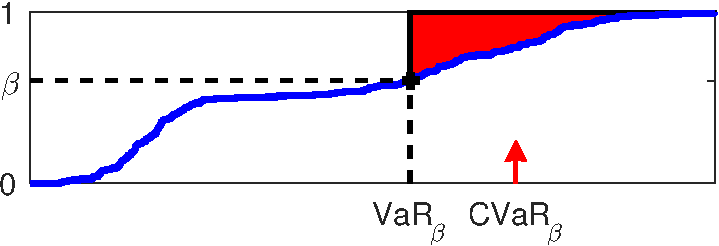
\includegraphics[width=0.25\textwidth]{figures/cvar}
\end{center}
\item CVaR is positively homogeneous, subadditive, monotone on $L^1$, and ``\textbf{translation equivariant}'': 
$
\mathrm{CVaR}[X + c] = \mathrm{CVaR}[X] + c
$
for any constant $c \in \mathbb R$.
\item CVaR has a convenient form for optimization:
\[
\mathrm{CVaR}_{\beta}[X] = 
\inf_{t \in \mathbb R} 
\left\{ 
t + \frac{1}{1-\beta} \mathbb E[(X - t)_+]\
\right\}
\]
\end{itemize}
\end{exampleblock}
\end{frame}

%%%%%%%%%%%%%%%%%%%%%%%%%%%%%%%%%%%%%%%%%%%%%%%%%

%%%%%%%%%%%%%%%%%%%%%%%%%%%%%%%%%%%%%%%%%%%%%%%%%
% \subsection{The Conditional Value-at-Risk}
% \begin{frame}\frametitle{Basic Properties and Reformulations}
% \visible<1->{
% \begin{exampleblock}{}
% \begin{itemize}
% \item A risk measure  $\risk : L^1(\Omega,\cF,\bbp) \to \overline{\mathbb R}$ that is\\ \textbf{-convex,\\ -positively homogeneous,\\ -monotonic}\\  \textbf{-translation equivariant} (p. 46)\\ is said to be \textbf{coherent}.
% \item $\CVaR_{\beta}$ is coherent.
% \end{itemize}
% \end{exampleblock}
% }
% \visible<2->{
% \begin{exampleblock}{}
% \begin{itemize}
% \item Coherent risk measures are \alert{distributionally robust} wrt the nominal measure $\bbp$. 
% \item What does that mean and why should I care?
% \end{itemize}
% \end{exampleblock}
% }
% \end{frame}


% \begin{frame}\frametitle{Distributional Robustness and CVaR}
% \begin{exampleblock}{}
% \begin{itemize}
% \item Return to risk neutral case $\risk = \mathbb E$. \alert{$\bbp$ is unknown}, but an iid sample is available.
% \item  We could use the \textbf{empirical probability measure} $\mathbb P_N$ and consider
% \[
% \min_{z \in \Zad} \wp(z) + \frac{1}{N} \sum_{i=1}^{N} \cJ(S(z))(\omega^i).
% \]
% \item This is a risk-neutral formulation, but expect \alert{overfitting}.
% \item We could \alert{incorporate risk aversion} by defining a set of measures 
% $
% \mathfrak{A} \subset \mathcal{P}(\Omega),
% $
% where $\mathcal{P}(\Omega)$ is the set of all Borel probability measures over $(\Omega,\cF)$, that contains $\mathbb P_{N}$.
% \item A robust data-driven formulation would then be
% \[
% \min_{z \in \Zad} \wp(z) + \sup_{\mathbb Q \in \mathfrak{A}}\mathbb E_{\mathbb Q}\left[ \cJ(S(z))\right].
% \]
% \end{itemize}
% \end{exampleblock}
% \end{frame}

% \begin{frame}\frametitle{Distributional Robustness and CVaR}
% \begin{exampleblock}{}
% \centering 
%  What is the ``\alert{correct}'' set $\mathfrak{A}$?
% \end{exampleblock}
% \visible<2->{
% \begin{exampleblock}{Examples}
% \begin{itemize}
% \item Let $\mathfrak{F}$ be a subset of integrands $f: \Omega \to \mathbb R$. 
% \item For $\varepsilon > 0$
% \[
% \mathfrak{A} := \left\{ \mathbb Q \in \mathcal{P}(\Omega) : \sup_{f \in \mathfrak{F}} \left| \mathbb E_{\mathbb P_{N}}[f] - \mathbb E_{\mathbb Q}[f]\right| \le \varepsilon
% \right\}
% \]
% \item Depending $\mathfrak{F}$ this is, e.g., a Wasserstein-1, Fortet-Mourier, or bounded Lipschitz metric.
% \item Without further insight, it is hard to see how this connects back to the theory of risk measures.
% \item The metrics do have the advantage that the support (atoms) can be moved.  
% \item The more tractable metrics, e.g., Wasserstein, are defined with integrands that have very little to do with the original integrand $\cJ(S(z))$.
% \end{itemize}
% \end{exampleblock}
% }
% \end{frame}

% \begin{frame}\frametitle{Distributional Robustness and CVaR}
% \vspace{-1ex}
% \begin{exampleblock}{}
% \begin{itemize}
% \item Using convex analysis, it can be shown in general that
% $
% \CVaR{\beta}[X] = \sup_{\vartheta \in \mathfrak{A}} \mathbb E_{\mathbb P}[\vartheta X],
% $
% where 
% \[
% \mathfrak{A} = \left\{\vartheta \in L^{\infty}(\Omega,\cF,\bbp) \; \left| \; \mathbb E_{\mathbb P}[\vartheta] = 1,\quad 0 \le \vartheta \le \frac{1}{1-\beta} \quad \mathbb P\textrm{-a.s.}\right.\right\}
% \]
% \item For $\bbp = \bbp_N$ we have
% $
% \mathfrak{A} = \left\{ \vartheta \in \mathbb R^{N} \; \left| \; \sum_{i=1}^{N} \frac{\vartheta_i}{N} = 1,\quad 0 \le \vartheta_i \le \frac{1}{1-\beta} \quad i=1,\dots,N \right.\right\}.
% $
% \item This implies 
% \[
% \CVaR{\beta}[X] = \sup_{\vartheta}\left\{ \frac{1}{N} \sum_{i=1}^{N} \vartheta_i X(\omega^i) :  \sum_{i=1}^{N} \frac{\vartheta_i}{N} = 1,\quad 0 \le \vartheta_i \le \frac{1}{1-\beta} \quad i=1,\dots,N\right\}
% \]
% \item CVaR can therefore be used in a data-driven distributionally robust setting.
% \item The original weights on $\mathbb P_N$ are readjusted to  $\vartheta_i/N$. 
% \item Our risk preference, expressed by $\CVaR{\beta}$, determines a meaningful set of probability measures.
% \end{itemize}
% \end{exampleblock}
% \end{frame}
%%%%%%%%%%%%%%%%%%%%%%%%%%%%%%%%%%%%%%%%%%%%%%%%%

%%%%%%%%%%%%%%%%%%%%%%%%%%%%%%%%%%%%%%%%%%%%%%%%%
% \begin{frame}\frametitle{}
% \begin{center}\Large
% Section 3: \\
% Optimization under Uncertainty in $\infty$-Dimensions \\
% Part I: Computing Consistent Gradients
% \end{center}
% \end{frame}
%%%%%%%%%%%%%%%%%%%%%%%%%%%%%%%%%%%%%%%%%%%%%%%%%



%%%%%%%%%%%%%%%%%%%%%%%%%%%%%%%%%%%%%%%%%%%%%%%%%
\subsection{Algorithms and Numerical Solution}

\begin{frame}\frametitle{}
\begin{center}\Large
Section 1\\
Part V:\\
Algorithms: Computing derivatives and treating uncertainty
\end{center}
\end{frame}

% \begin{frame}\frametitle{How can I solve the optimization problem numerically?}
% \begin{block}{}
% As mentioned above, there are two approaches
% \begin{itemize}
% \item Reduced space approach
% \item Full space approach
% \end{itemize}
% \end{block}

% \begin{block}{}\centering
% We highlight the main points for the \textbf{deterministic reduced space} approach.
% \end{block}

% \begin{block}{}\centering
% The full space approach is especially important for PDEs with non-unique solutions, e.g., stationary Allen-Cahn (p. 17 above).
% \end{block}
% \end{frame}

\begin{frame}\frametitle{OUU in $\infty$-Dimensions?}
\visible<1->{
\vspace{-1ex}
\begin{exampleblock}{}
\begin{itemize}
%\item For the moment,  ignore the PDEs and random inputs.
\item We are interested in composite optimization problems of the type:
\vspace{-2ex}
\[ 
\min_{x \in X_{\rm ad}} f(x) + \Phi(F(x)) \text{ over } x \in X.
\]\vspace{-2ex}
\item $X, Y$ are real \textbf{Hilbert spaces}. 
\item $f:X \to \mathbb R$ is typically continuous, convex, \textbf{differentiable}.
\item $\Phi: Y \to \mathbb R$ is \textbf{nonsmooth}, convex, positive homogeneous, monotone.
\item $F: X \to Y$ is continuous, typically differentiable, \textbf{expensive to evaluate}.
\end{itemize}
\end{exampleblock}
}
\visible<2->{
\begin{exampleblock}{}
\begin{itemize}
\item \visible<2->{
\textbf{``PDE''-part}: $X$ replaces $\{X_h\}$, $X_h$  finite dim.\ with elements $u_{h}(x) = \sum_{i=1}^{N} u^h_i \varphi^h_i(x)$.
}
\item \visible<3->{
\textbf{``PDE''-part}: $F(x)$ requires the solution of a PDE with input $x$.
}
\item \visible<4->{
\textbf{``Random"-part}: cannot evaluate $F(x)$ or even $F(x_h)$ $x_h \in X_h$.
}
\item \visible<5->{Derivatives are \textbf{dual} objects, gradients are \textbf{primal}.
}
\item \visible<6->{To compute $x_{k} - \gamma_k\nabla f(x_k)$ in an algorithm, we first need
 $\nabla f(x) = \mathfrak{R}_{\rm Riesz} f'(x)$.}
%\item $R^{-1}_{\rm Riesz}$ is usually not the identity {\rm Id}; may require a PDE solve.
\end{itemize}
\end{exampleblock}
}
\end{frame}

\begin{frame}\frametitle{Riesz Mappings}
\begin{example}
\begin{itemize}
\item 
\visible<1->{
Let $D \subset \mathbb R^n$ be open and bounded. Let $A \subset D$ be Lebesgue measurable with $|A| > 0$.
}
\item 
\visible<2->{
For $x \in D$, set $\varphi(x) = 1$ if $x \in A$ and $0$ otherwise.
}
\item 
\visible<3->{
Since $H^1_0(D) \subset L^2(D)$ and $\varphi$ is bounded and measurable, we see that 
\[
H^1_0(D) \ni u \mapsto (\varphi, u)_{L^2(D)}
\]
defines a bounded linear functional on $H^1_0(D)$.
}
\item 
\visible<4->{
We can therefore identity $\varphi$ with an element of $H^{-1}(D) = (H^1_0(D))^*$.
}
\item 
\visible<5->{
It's tempting to make the \alert{fallacious argument}:  
\begin{center}
\textit{$H^1_0(D)$ is a Hilbert space, I can just identify it with its dual and treat elements in $H^{-1}(D)$ like they are in $H^1_0(D)$.}
\end{center}
}
\item \visible<6->{ But $\varphi$ will have \textbf{jumps} in general, so $\varphi \not\in H^1_0(D)$!
}
\end{itemize}
\end{example}
\end{frame}

\begin{frame}\frametitle{Riesz Mappings}
\begin{example}
\begin{itemize}
\item 
\visible<1->{The \textbf{Riesz Representation Theorem} states: Let $H$ be a real Hilbert space and $\varphi \in H^*$ (the topological dual of $H$). Then there exists a unique element $u_{\varphi} \in H$ such that 
\[
\langle \varphi, v \rangle_{H^*,H} = (u_{\varphi}, v)_{H} \quad \forall v \in H\text{ and } 
\|\varphi\|_{H^*} = \|u_{\varphi} \|_{H}
\]
}\vspace{-4ex}
\item \visible<2->{...so if $\varphi$ above is in $H^{-1}(D)$, then there exists a unique $u_{\varphi} \in H^1_0(D)$ such that
\[
(u_{\varphi}, v)_{H^1_0(D)} = \langle \varphi, v \rangle_{H^{-1}(D),H^1_0(D)} \quad \forall v \in H^1_0(D).
\]
}\vspace{-4ex}
\item \visible<3->{Since 
$
(u_{\varphi}, v)_{H^1_0(D)} = (\nabla u_{\varphi}, \nabla v)_{L^2(D)}$ $\forall v \in H^1_0(D), 
$ we have
\[
u_{\varphi} = (-\Delta)^{-1} \varphi,
\]
i.e., $\mathfrak{R}_{\rm Riesz}$ requires the solution of Poisson problem in $H^1_0(D)$.
}
\end{itemize}
\end{example}
\end{frame}

\begin{frame}\frametitle{Using the Correct Discrete Gradients}
\vspace{-2ex}
\begin{example}[]
\begin{itemize}
\item
$f : L^2(D) \to \mathbb R$  is defined via continuous bilinear form.
\item 
$X_h \subset L^2(D)$ is a finite dim.\ subspace defined by the nodal basis from the FEM. 
\item 
$u_h \in X_h$ is associated with coefficient vector $\mathbf{u}_h \in \mathbb R^n$ \pause
\item 
$f_h : \mathbb R^n \to \mathbb R$ is the FE discretization of $f$, e.g.
\[
f_h(\mathbf{u}_h) = \frac{1}{2} \mathbf{u}^T_h L_h \mathbf{u}_h
\]
\item The correct gradient for a numerical approach would then be
\[
\mathfrak{R}_{L^2}(f_h'(\mathbf{u}_h)) = M_h^{-1} L_h \mathbf{u}_h.
\]
$M_h$ is the mass matrix associated with the discrete $L^2$-inner product.
\item If $f(u) = (u,u)_{L^2(D)}$, then $\mathfrak{R}_{L^2}(f_h'(\mathbf{u}_h))$ is just the \textbf{vector of nodal values} $\bm u_h$, \alert{not} $M_h \bm u_h$!
\end{itemize}
\end{example}
\end{frame}


\begin{frame}\frametitle{Two essential computations}
\begin{exampleblock}{}
\begin{itemize}
\item How do we efficiently \textbf{compute gradients} in the reduced space setting?
\item How do we efficiently \textbf{compute Hessian-vector products} in the reduced space setting?
% \item The PDE is now implicitly satisfied. 
% \item There may still exist control and state constraints.
% \item The PDE-constraint is formulated in function spaces $U, Z, W$, which are typically Hilbert spaces; in some settings general Banach spaces.
% \item Efficient algorithms need to be ``aware'' of the original function spaces:
% \begin{enumerate}
% \item Inner products, dual norms, etc. should be implemented with the proper discrete counterpart.
% \item Gradients/Hessians of the objective, constraints, and solution operators should be calculated using the associated discrete Riesz mappings.
% \end{enumerate}
% \item This ensures (usually) \textbf{mesh independent} behavior and proper \textbf{scaling} by mesh refinements.
\end{itemize}
\end{exampleblock}

\visible<2->{
\begin{exampleblock}{}
\begin{itemize}
    \item We only discuss the deterministic case.
    % \item These are essential for all competitive optimization algorithms.
    \item The \textbf{Hessian} is \alert{never} available, but \textbf{Hessian-vector products} allow us to apply \textbf{Newton's method} and its variants.
\end{itemize}
\end{exampleblock}
}
\end{frame}

\begin{frame}\frametitle{Computing the Gradient}
\begin{exampleblock}{}
\begin{itemize}
\visible<1->{
\item Given $z \in Z$, calculate \textbf{state} $u = S(z)$ by solving $e(u,z) = 0$.
}
\visible<2->{
\item Given $u$, solve \textbf{adjoint equation} for $\lambda = P(z)$: $e_{u}(u,z)^* \lambda = -J'_u(u,z)$.
}
\visible<3->{
\item Given $z,u,\lambda$ calculate the full gradient 
\[
\nabla \mathcal{J}(z) = e_{z}(u,z)^* \lambda + \nabla J_u(u,z).\pause
\]
}\vspace{-3ex}
\visible<4->{
\item This might require an additional solve for the true discrete gradient.
}
\visible<5->{
\item In the linear case, we only require the solution of \textbf{sparse structured linear} systems for $\nabla \mathcal{J}$.
}
\visible<6->{
\item Without \textbf{adjoints}, $\nabla \mathcal{J}$ would contain \alert{large dense matrices} due to the solution operators $S, P$.
}
\end{itemize}
\end{exampleblock}
\end{frame}

\begin{frame}\frametitle{Hessian-Vector Products}
\begin{exampleblock}{}
\begin{itemize}
\visible<1->{
\item Define the Lagrangian $L(u,z,\lambda)$:
$
L(u,z,\lambda) = J(u,z) + \langle e(u,z), \lambda \rangle_{W,W^*}
$
}
\visible<2->{
\item Given $z \in Z$, calculate $u = S(z)$ by solving $e(u,z) = 0$.
}
\visible<3->{
\item Given $u$, solve the adjoint equation for $\lambda = P(z)$: $e_{u}(u,z)^* \lambda = -J'_u(u,z)$
}
\visible<4->{
\item Given $u,z$, direction $v$, solve the \textbf{state sensitivity equation} for $w$:
\[
e_u(u,z) w = e_z(u,z)v.
\]
}\vspace{-4ex}
\visible<5->{
\item  Given $u,z,\lambda,w,v$ solve the \textbf{adjoint sensitivity equation} for $p$:
\[
e_{u}(u,z)^* p = L''_{uu}(u,z,\lambda)w - L''_{uz}(u,z,\lambda)v.
\]
}\vspace{-4ex}
\visible<6->{
\item Given $u,z,\lambda,w,v,p$ yields
\[
\nabla^2 \mathcal{J}(z) v = e_{z}(u,z)^*p - \nabla_{zu} L(u,z,\lambda)w + \nabla_{zz} L(u,z,\lambda) v.
\]\vspace{-4ex}
}
\end{itemize}
\end{exampleblock}
\end{frame}

\begin{frame}\frametitle{Uncertainty in Computation}
\begin{exampleblock}{}
% There are essentially two possibilities (assume for now $\risk = \mathbb E$)
\begin{itemize}
\item \textbf{Sample-before-you-go:} \textbf{Replace} underlying $\mathbb P$ by  \textbf{approximation} $\mathbb P_N$ solve
\[
\min_{z \in Z_{\rm ad}} \mathbb E_{\mathbb P_N(\cdot)}[\mathcal{J}(S(z))] = \frac{1}{N}\sum_{i=1}^{N} \mathcal{J}(S(z))(\omega^i)
\]
\visible<2->{
\item \textbf{Sample-while-you-go:} Given positive step sizes $\{\gamma_i\}_{i=1}^N$ approximate the solution $z^{\star}$ using \textbf{stochastic gradients}
\[
G_i :=  S'(z_i,\omega^i)^* \nabla \mathcal{J}(S(z^i,\omega^i)) \quad i=1,\dots,N
\]
with a sequence $\{z^i\}$ given by (for example)
\[
z^{i+1} = \mathrm{Proj}_{Z_{\rm ad}}(z^i - \gamma^i G_i).
\]
% \item Batches and second-order information can be incorporated. 
}
\end{itemize}
\end{exampleblock}
\end{frame}

\begin{frame}\frametitle{Uncertainty in Computation}
\begin{exampleblock}{}
\begin{itemize}
\item ``Sample-before-you-go'' covers all manner of empirical approximations: Monte Carlo, Quasi-Monte Carlo, Deterministic Quadrature, Sparse Grids ... 
\item Sometimes called Sample Average Approximation (SAA)
\item I will use the term \textbf{Empirical Approximation}.
\item Yields a deterministic PDE-constrained problem that can be solved with existing approaches.
\item \textbf{These are not optimization algorithms.}
\end{itemize}
\end{exampleblock}
\visible<2->{
\begin{exampleblock}{}
\begin{itemize}
\item ``Sample-while-you-go'' has its origins in \textbf{Stochastic Approximation}. 
\item I will use the term \textbf{Stochastic Approximation}.
\item Many variants with different step size rules, half-steps, extrapolations, etc.
\item Immensely popular in machine learning
\item \textbf{These are (typically first-order) algorithms.}
\end{itemize}
\end{exampleblock}
}
\end{frame}


\begin{frame}\frametitle{Stopping Criteria}
\begin{exampleblock}{}
\begin{itemize}
\item \textbf{When} to stop with \textbf{sample-before-you-go}: Use optimality conditions.
\visible<2->{
\item Define
\[
\mathrm{res}_k := z_{k} - \mathrm{Proj}_{\Zad}(z_{k} - \mathbb E_{\bbp_{N}}\left[\cJ(S(z_{k}))\right])
\]
and stop when
\[
\| \mathrm{res}_{k} \|
\le
\tau_{\rm rel}\| \mathrm{res}_{0} \| + \tau_{\rm abs},
\]
where $\tau_{\rm rel} > 0$ and $\tau_{\rm abs} > 0$ are absolute and relative tolerances, respectively.
}
\visible<3->{
\item Knowing \textbf{when} to stop the \textbf{sample-as-you-go} algorithms is more difficult.
}
\visible<4->{
\item The  basic convergence theory usually only provides statements on the objective functions. 
}
\visible<5->{
\item In \alert{both} settings, the ``solution'' $z^{\star}(\bbp_{N})$ is \alert{dependent on the realization of random processes}. 
}
\visible<6->{
\item Ideally, we would know what happens to $z^{\star}(\mathbb P_{N})$ as $N \to +\infty$. More on this later...
}
\end{itemize}
\end{exampleblock} 
\end{frame}
%%%%%%%%%%%%%%%%%%%%%%%%%%%%%%%%%%%%%%%%%%%%%%%%%



%%%%%%%%%%%%%%%%%%%%%%%%%%%%%%%%%%%%%%%%%%%%%%%%%
%%%%%%%%%%%%%%%%%%%%%%%%%%%%%%%%%%%%%%%%%%%%%%%%%
% \section{Risk-Averse Decision Making}
%%%%%%%%%%%%%%%%%%%%%%%%%%%%%%%%%%%%%%%%%%%%%%%%%
%%%%%%%%%%%%%%%%%%%%%%%%%%%%%%%%%%%%%%%%%%%%%%%%%

%%%%%%%%%%%%%%%%%%%%%%%%%%%%%%%%%%%%%%%%%%%%%%%%%
% \begin{frame}\frametitle{}
% \begin{center}\Large
% Section 2: \\
% Risk-Averse Decision Making 
% \end{center}
% \end{frame}
% %%%%%%%%%%%%%%%%%%%%%%%%%%%%%%%%%%%%%%%%%%%%%%%%%

% %%%%%%%%%%%%%%%%%%%%%%%%%%%%%%%%%%%%%%%%%%%%%%%%%
% \subsection{Risk Models}
% \begin{frame}\frametitle{Robust Optimization}
% \visible<1->{
% \begin{exampleblock}{Motivation}
% \begin{itemize}
% \item An \textbf{uncertainty region} $\Omega$ is known, but \alert{no data} for statistical estimation is available.
% \item An \textbf{uncertainty region} $\Omega$ is known and data is available, but there is \alert{no room for error}.
% \item An \textbf{uncertainty region} $\Omega$ is known and data is available, but the \alert{$\mathrm{dim}\, \Omega$ is intractable}.
% \item The functional $\risk$ should then take the form  
% \[
% \risk[X] := \sup_{\omega \in \Omega} X(\omega).
% \]
% \end{itemize}
% \end{exampleblock}
% }
% \visible<2->{
% \begin{exampleblock}{}
% \begin{itemize}
% \item The robust PDE-constrained optimization problem takes the general form:
% \begin{equation}\label{eq:robust}
% \min_{z \in \Zad}\left\{ \wp(z) + \sup_{\omega \in \Omega} \mathcal{J}(S(z))(\omega) \right\}
% \end{equation}
% \item \alert{Hard to solve}: A nonsmooth, possibly nonconvex, $\infty$-dimensional problem. 
% % %\item The formulation might be overly restrictive/too pessimistic.
% % \item Existing approaches transform \eqref{eq:robust} into a mathematical program with equilibrium constraints (MPEC). MPECs with PDE operators are very hard to solve numerically.
% \end{itemize}
% \end{exampleblock}
% }
% \end{frame}

% \begin{frame}\frametitle{Stochastic Order Constraints}
% \vspace{-2ex}
% \begin{exampleblock}{Motivation}
% \begin{itemize}
% \visible<1->{
% \item A \textbf{complete probability space} $(\Omega,\cF, \bbp)$ is available.
% \item A \textbf{benchmark} decision, design, stationary control $z_d \in Z$ or objective value $c$ is given.
% }
% \visible<2->{
% \item The risk-averse PDE-constrained optimization problem might take the general form:
% \begin{equation}\label{eq:prob}
% \min_{z \in \Zad} \left\{ \wp(z) + \mathbb E \left[\mathcal{J}(S(z)) \right] : \mathbb P\left\{\cJ(S(z)) < \cJ(S(z_{d}))\right\} \ge p \right\} \quad p \in (0,1).\vspace{-4ex}
% \end{equation}
% }
% \end{itemize}
% \visible<3->{
% \begin{center}
%     \textit{Find $z^{\star} \in \Zad$ that \alert{performs well on average} such that the random variable $\omega \mapsto \mathcal{J}(S(z^{\star}))(\omega) - \cJ(S(z_{d}))(\omega)$ is \alert{negative with probability $p$.}
%     }    
% \end{center}
% }
% \end{exampleblock}
% \visible<4->{
% \begin{exampleblock}{}
% Many variants available: 
% \begin{itemize}
% \item Replace $\cJ(S(z_{d}))$ with a constant $c$ or choose more than one/all $p \in (0,1)$.
% \item Compare \alert{tails}  of $\cJ(S(z))$ to $\cJ(S(z_{d}))$ over a range of values.
% \item The constraint function $\varphi(z) := \mathbb P\left\{\cJ(S(z)) \le c \right\}$ is highly nontrivial.
% \end{itemize}
% \end{exampleblock}
% }
% \end{frame}


% \begin{frame}\frametitle{Minimizing the Expectation}
% \visible<1->{
% \begin{exampleblock}{Optimization with Risk Measures}
% \begin{itemize}
% \item The risk-averse PDE-constrained optimization problem takes the general form:
% \begin{equation}\label{eq:prob}
% \min_{z \in \Zad} \left\{ \wp(z) + \risk \left[\mathcal{J}(S(z)) \right] \right\}
% \end{equation}
% \item $\risk$ should ``shape'' the distribution of the objective function at an optimal solution $z^{\star}$. 
% \end{itemize}
% \end{exampleblock}
% }
% \visible<2->{
% \begin{exampleblock}{Traditional Approach: $\risk = \mathbb E$ (``risk neutral case'')}
% \begin{itemize}
% \visible<2->{
% \item Optimize to achieve best performance \textbf{on average}.
% \item Q: \alert{What could possibly go wrong?} 
% }
% \visible<3->{\item A: Does not account for potentially catastrophic tail events.}
% \visible<4->{\item Often consider: $\nu \bbe + (1-\nu) \risk$ with $\risk$ being something other than $\mathbb E$, $\nu \in (0,1)$, instead.}
% \end{itemize}
% \end{exampleblock}
% }
% \end{frame}

% \begin{frame}\frametitle{Mitigating Risk using Risk Measures}


% \begin{exampleblock}{Traditional Mean-Var Approach: $\risk = \nu \mathbb E+(1-\nu) \mathbb V$}
% \begin{itemize}
% \visible<1->{
% \item Maximize \textbf{average performance} vs.\ \textbf{minimize variance} $\mathbb V[X] = \mathbb E[(X-\mathbb E[X])^2]$ 
% \item Q: \alert{What could possibly go wrong?} 
% }
% \visible<2->{
% \item A:  $\mathbb V$ may penalize favorable outlier situations: We are happy if $\cJ(S(z))(\omega) \ll \cJ(S(y))(\omega)$.
% \item $\mathbb V$ is not monotone w.r.t.\ the partial order on ${L}^{1}(\Omega,\cF, \bbp)$: The pointwise bound
% \[
% \cJ(S(z))(\omega) \le \cJ(S(y))(\omega),\; \Pae \omega \in \Omega
% \]
% does not guarantee $\mathbb V(\cJ(S(z))) \le \mathbb V(\cJ(S(y)))$. 
% \item This is not seen to be favorable for optimization.
% }
% \end{itemize}
% \end{exampleblock}
% \end{frame}

% \begin{frame}\frametitle{Mitigating Risk using Risk Measures}
% \begin{exampleblock}{Minimize the $\beta$-Quantile: $\risk[X] = \inf\{ \tau : \bbp(X \le \tau) \ge \beta \} $}
% \begin{itemize}
% \visible<1->{
% \item Also know as \textbf{Value-at-Risk} (confidence/risk level $\beta \in (0,1)$).
% \item Smallest $\tau$ such that with probability $\beta$, $\cJ(S(z))$ does not exceed the value $\tau$.  
% \item Measures risky (catastrophic) events.
% }
% \item Q: \alert{What could possibly go wrong?} 
% \visible<2->{
% \item A: $\mathrm{VaR}$ does not account for the size of the tail. 
% \item A:  $\mathrm{VaR}$ is not subadditive. 
% \item Obviously difficult to minimize in general.
% }
% \end{itemize}
% \end{exampleblock}
% \end{frame}

% \begin{frame}\frametitle{Mitigating Risk using Risk Measures}
% \vspace{-2ex}
% \begin{exampleblock}{Minimize the $\beta$-Average $\mathrm{VaR}$: $\risk[X] := \frac{1}{1-\beta}\int_{\beta}^{1} \mathrm{VaR}_{\alpha}[X] \mathrm{d}\alpha$}
% \begin{itemize}
% \visible<1->{
% \item Many names:  Excess Loss, Mean Shortfall, Average VaR, Tail VaR. 
% \item We use \textbf{Conditional Value-at-Risk} ($\mathrm{CVaR}$).
% \item Minimize the expectation of the tail above the $\beta$-quantile.
% \begin{center}
% }
% 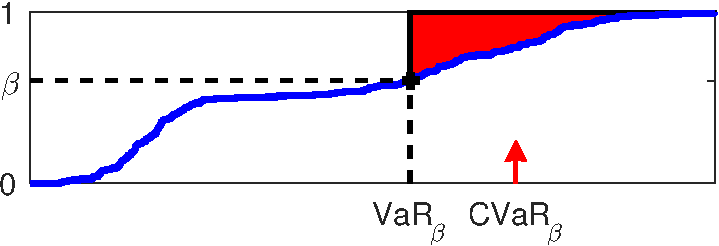
\includegraphics[width=0.25\textwidth]{figures/cvar}
% \end{center}
% \item CVaR is positively homogeneous, subadditive, monotone on $L^1$, and ``\textbf{translation equivariant}'': 
% $
% \mathrm{CVaR}[X + c] = \mathrm{CVaR}[X] + c
% $
% for any constant $c \in \mathbb R$.
% \item CVaR has a convenient form for optimization:
% \[
% \mathrm{CVaR}_{\beta}[X] = 
% \inf_{t \in \mathbb R} 
% \left\{ 
% t + \frac{1}{1-\beta} \mathbb E[(X - t)_+]\
% \right\}
% \]
% \end{itemize}
% \end{exampleblock}
% \end{frame}

%%%%%%%%%%%%%%%%%%%%%%%%%%%%%%%%%%%%%%%%%%%%%%%%%

%%%%%%%%%%%%%%%%%%%%%%%%%%%%%%%%%%%%%%%%%%%%%%%%%
% \subsection{The Conditional Value-at-Risk}
% \begin{frame}\frametitle{Basic Properties and Reformulations}
% \visible<1->{
% \begin{exampleblock}{}
% \begin{itemize}
% \item A risk measure  $\risk : L^1(\Omega,\cF,\bbp) \to \overline{\mathbb R}$ that is\\ \textbf{-convex,\\ -positively homogeneous,\\ -monotonic}\\  \textbf{-translation equivariant} (p. 46)\\ is said to be \textbf{coherent}.
% \item $\CVaR_{\beta}$ is coherent.
% \end{itemize}
% \end{exampleblock}
% }
% \visible<2->{
% \begin{exampleblock}{}
% \begin{itemize}
% \item Coherent risk measures are \alert{distributionally robust} wrt the nominal measure $\bbp$. 
% \item What does that mean and why should I care?
% \end{itemize}
% \end{exampleblock}
% }
% \end{frame}


% \begin{frame}\frametitle{Distributional Robustness and CVaR}
% \begin{exampleblock}{}
% \begin{itemize}
% \item Return to risk neutral case $\risk = \mathbb E$. \alert{$\bbp$ is unknown}, but an iid sample is available.
% \item  We could use the \textbf{empirical probability measure} $\mathbb P_N$ and consider
% \[
% \min_{z \in \Zad} \wp(z) + \frac{1}{N} \sum_{i=1}^{N} \cJ(S(z))(\omega^i).
% \]
% \item This is a risk-neutral formulation, but expect \alert{overfitting}.
% \item We could \alert{incorporate risk aversion} by defining a set of measures 
% $
% \mathfrak{A} \subset \mathcal{P}(\Omega),
% $
% where $\mathcal{P}(\Omega)$ is the set of all Borel probability measures over $(\Omega,\cF)$, that contains $\mathbb P_{N}$.
% \item A robust data-driven formulation would then be
% \[
% \min_{z \in \Zad} \wp(z) + \sup_{\mathbb Q \in \mathfrak{A}}\mathbb E_{\mathbb Q}\left[ \cJ(S(z))\right].
% \]
% \end{itemize}
% \end{exampleblock}
% \end{frame}

% \begin{frame}\frametitle{Distributional Robustness and CVaR}
% \begin{exampleblock}{}
% \centering 
%  What is the ``\alert{correct}'' set $\mathfrak{A}$?
% \end{exampleblock}
% \visible<2->{
% \begin{exampleblock}{Examples}
% \begin{itemize}
% \item Let $\mathfrak{F}$ be a subset of integrands $f: \Omega \to \mathbb R$. 
% \item For $\varepsilon > 0$
% \[
% \mathfrak{A} := \left\{ \mathbb Q \in \mathcal{P}(\Omega) : \sup_{f \in \mathfrak{F}} \left| \mathbb E_{\mathbb P_{N}}[f] - \mathbb E_{\mathbb Q}[f]\right| \le \varepsilon
% \right\}
% \]
% \item Depending $\mathfrak{F}$ this is, e.g., a Wasserstein-1, Fortet-Mourier, or bounded Lipschitz metric.
% \item Without further insight, it is hard to see how this connects back to the theory of risk measures.
% \item The metrics do have the advantage that the support (atoms) can be moved.  
% \item The more tractable metrics, e.g., Wasserstein, are defined with integrands that have very little to do with the original integrand $\cJ(S(z))$.
% \end{itemize}
% \end{exampleblock}
% }
% \end{frame}

% \begin{frame}\frametitle{Distributional Robustness and CVaR}
% \vspace{-1ex}
% \begin{exampleblock}{}
% \begin{itemize}
% \item Using convex analysis, it can be shown in general that
% $
% \CVaR{\beta}[X] = \sup_{\vartheta \in \mathfrak{A}} \mathbb E_{\mathbb P}[\vartheta X],
% $
% where 
% \[
% \mathfrak{A} = \left\{\vartheta \in L^{\infty}(\Omega,\cF,\bbp) \; \left| \; \mathbb E_{\mathbb P}[\vartheta] = 1,\quad 0 \le \vartheta \le \frac{1}{1-\beta} \quad \mathbb P\textrm{-a.s.}\right.\right\}
% \]
% \item For $\bbp = \bbp_N$ we have
% $
% \mathfrak{A} = \left\{ \vartheta \in \mathbb R^{N} \; \left| \; \sum_{i=1}^{N} \frac{\vartheta_i}{N} = 1,\quad 0 \le \vartheta_i \le \frac{1}{1-\beta} \quad i=1,\dots,N \right.\right\}.
% $
% \item This implies 
% \[
% \CVaR{\beta}[X] = \sup_{\vartheta}\left\{ \frac{1}{N} \sum_{i=1}^{N} \vartheta_i X(\omega^i) :  \sum_{i=1}^{N} \frac{\vartheta_i}{N} = 1,\quad 0 \le \vartheta_i \le \frac{1}{1-\beta} \quad i=1,\dots,N\right\}
% \]
% \item CVaR can therefore be used in a data-driven distributionally robust setting.
% \item The original weights on $\mathbb P_N$ are readjusted to  $\vartheta_i/N$. 
% \item Our risk preference, expressed by $\CVaR{\beta}$, determines a meaningful set of probability measures.
% \end{itemize}
% \end{exampleblock}
% \end{frame}
%%%%%%%%%%%%%%%%%%%%%%%%%%%%%%%%%%%%%%%%%%%%%%%%%

%%%%%%%%%%%%%%%%%%%%%%%%%%%%%%%%%%%%%%%%%%%%%%%%%
% \begin{frame}\frametitle{}
% \begin{center}\Large
% Section 3: \\
% Optimization under Uncertainty in $\infty$-Dimensions \\
% Part I: Computing Consistent Gradients
% \end{center}
% \end{frame}
%%%%%%%%%%%%%%%%%%%%%%%%%%%%%%%%%%%%%%%%%%%%%%%%%


%%%%%%%%%%%%%%%%%%%%%%%%%%%%%%%%%%%%%%%%%%%%%%%%%
%%%%%%%%%%%%%%%%%%%%%%%%%%%%%%%%%%%%%%%%%%%%%%%%%
\section{Algorithms for OUU}
%%%%%%%%%%%%%%%%%%%%%%%%%%%%%%%%%%%%%%%%%%%%%%%%%
%%%%%%%%%%%%%%%%%%%%%%%%%%%%%%%%%%%%%%%%%%%%%%%%%

% \subsection{Computing Consistent Gradients}
% \begin{frame}\frametitle{OUU in $\infty$-Dimensions?}
% \visible<1->{
% \vspace{-1ex}
% \begin{exampleblock}{}
% \begin{itemize}
% %\item For the moment,  ignore the PDEs and random inputs.
% \item We are interested in composite optimization problems of the type:
% \vspace{-2ex}
% \[ 
% \min_{x \in X_{\rm ad}} f(x) + \Phi(F(x)) \text{ over } x \in X.
% \]\vspace{-2ex}
% \item $X, Y$ are real \textbf{Hilbert spaces}. 
% \item $f:X \to \mathbb R$ is typically continuous, convex, \textbf{differentiable}.
% \item $\Phi: Y \to \mathbb R$ is \textbf{nonsmooth}, convex, positive homogeneous, monotone.
% \item $F: X \to Y$ is continuous, typically differentiable, \textbf{expensive to evaluate}.
% \end{itemize}
% \end{exampleblock}
% }
% \visible<2->{
% \begin{exampleblock}{}
% \begin{itemize}
% \item \visible<2->{
% \textbf{``PDE''-part}: $X$ replaces $\{X_h\}$, $X_h$  finite dim.\ with elements $u_{h}(x) = \sum_{i=1}^{N} u^h_i \varphi^h_i(x)$.
% }
% \item \visible<3->{
% \textbf{``PDE''-part}: $F(x)$ requires the solution of a PDE with input $x$.
% }
% \item \visible<4->{
% \textbf{``Random"-part}: cannot evaluate $F(x)$ or even $F(x_h)$ $x_h \in X_h$.
% }
% \item \visible<5->{Derivatives are \textbf{dual} objects, gradients are \textbf{primal}.
% }
% \item \visible<6->{To compute $x_{k} - \gamma_k\nabla f(x_k)$ in an algorithm, we first need
%  $\nabla f(x) = \mathfrak{R}_{\rm Riesz} f'(x)$.}
% %\item $R^{-1}_{\rm Riesz}$ is usually not the identity {\rm Id}; may require a PDE solve.
% \end{itemize}
% \end{exampleblock}
% }
% \end{frame}

% \begin{frame}\frametitle{Riesz Mappings}
% \begin{example}
% \begin{itemize}
% \item 
% \visible<1->{
% Let $D \subset \mathbb R^n$ be open and bounded. Let $A \subset D$ be Lebesgue measurable with $|A| > 0$.
% }
% \item 
% \visible<2->{
% For $x \in D$, set $\varphi(x) = 1$ if $x \in A$ and $0$ otherwise.
% }
% \item 
% \visible<3->{
% Since $H^1_0(D) \subset L^2(D)$ and $\varphi$ is bounded and measurable, we see that 
% \[
% H^1_0(D) \ni u \mapsto (\varphi, u)_{L^2(D)}
% \]
% defines a bounded linear functional on $H^1_0(D)$.
% }
% \item 
% \visible<4->{
% We can therefore identity $\varphi$ with an element of $H^{-1}(D) = (H^1_0(D))^*$.
% }
% \item 
% \visible<5->{
% It's tempting to make the \alert{fallacious argument}:  
% \begin{center}
% \textit{$H^1_0(D)$ is a Hilbert space, I can just identify it with its dual and treat elements in $H^{-1}(D)$ like they are in $H^1_0(D)$.}
% \end{center}
% }
% \item \visible<6->{ But $\varphi$ will have \textbf{jumps} in general, so $\varphi \not\in H^1_0(D)$!
% }
% \end{itemize}
% \end{example}
% \end{frame}

% \begin{frame}\frametitle{Riesz Mappings}
% \begin{example}
% \begin{itemize}
% \item 
% \visible<1->{The \textbf{Riesz Representation Theorem} states: Let $H$ be a real Hilbert space and $\varphi \in H^*$ (the topological dual of $H$). Then there exists a unique element $u_{\varphi} \in H$ such that 
% \[
% \langle \varphi, v \rangle_{H^*,H} = (u_{\varphi}, v)_{H} \quad \forall v \in H\text{ and } 
% \|\varphi\|_{H^*} = \|u_{\varphi} \|_{H}
% \]
% }\vspace{-4ex}
% \item \visible<2->{...so if $\varphi$ above is in $H^{-1}(D)$, then there exists a unique $u_{\varphi} \in H^1_0(D)$ such that
% \[
% (u_{\varphi}, v)_{H^1_0(D)} = \langle \varphi, v \rangle_{H^{-1}(D),H^1_0(D)} \quad \forall v \in H^1_0(D).
% \]
% }\vspace{-4ex}
% \item \visible<3->{Since 
% $
% (u_{\varphi}, v)_{H^1_0(D)} = (\nabla u_{\varphi}, \nabla v)_{L^2(D)}$ $\forall v \in H^1_0(D), 
% $ we have
% \[
% u_{\varphi} = (-\Delta)^{-1} \varphi,
% \]
% i.e., $\mathfrak{R}_{\rm Riesz}$ requires the solution of Poisson problem in $H^1_0(D)$.
% }
% \end{itemize}
% \end{example}
% \end{frame}

% \begin{frame}\frametitle{Using the Correct Discrete Gradients}
% \vspace{-2ex}
% \begin{example}[]
% \begin{itemize}
% \item
% $f : L^2(D) \to \mathbb R$  is defined via continuous bilinear form.
% \item 
% $X_h \subset L^2(D)$ is a finite dim.\ subspace defined by the nodal basis from the FEM. 
% \item 
% $u_h \in X_h$ is associated with coefficient vector $\mathbf{u}_h \in \mathbb R^n$ \pause
% \item 
% $f_h : \mathbb R^n \to \mathbb R$ is the FE discretization of $f$, e.g.
% \[
% f_h(\mathbf{u}_h) = \frac{1}{2} \mathbf{u}^T_h L_h \mathbf{u}_h
% \]
% \item The correct gradient for a numerical approach would then be
% \[
% \mathfrak{R}_{L^2}(f_h'(\mathbf{u}_h)) = M_h^{-1} L_h \mathbf{u}_h.
% \]
% $M_h$ is the mass matrix associated with the discrete $L^2$-inner product.
% \item If $f(u) = (u,u)_{L^2(D)}$, then $\mathfrak{R}_{L^2}(f_h'(\mathbf{u}_h))$ is just the \textbf{vector of nodal values} $\bm u_h$, \alert{not} $M_h \bm u_h$!
% \end{itemize}
% \end{example}
% \end{frame}

% \begin{frame}\frametitle{Using the Correct Discrete Gradients}
% \begin{example}[]
% \begin{itemize}
% \item \visible<1->{
% Suppose $f : L^2(D) \to \mathbb R$ is defined
% \[
% f(u) := 
% \frac{1}{2}\int_{\Omega} ( L(\xi(\omega)) u, u )_{L^2(D)} \, \mathrm{d} \mathbb P(\omega),
% \]
% where $\xi : (\Omega, \mathcal{F}, \mathbb P) \to \mathbb R^d$ is a random vector.}
% \item \visible<2->{Given an iid sample $\xi^1,\dots,\xi^N$ we would use
% $
% f_N(u) := \frac{1}{2N} \sum_{i=1}^N ( L(\xi^i) u, u )_{L^2(D)}.
% $
% % in \textbf{empirical approximations} of $\mathbb P$.
% }
% \item \visible<3->{The correct fully discrete gradient would then be \vspace{-1ex}
% \[
% \mathfrak{R}_{L^2}(f_{N,h}'(\mathbf{u}_h)) = \frac{1}{N} \sum_{i=1}^N M_h^{-1} L^{i}_h \mathbf{u}_h,
% \vspace{-1ex}
% \]
% where 
% $
% \mathbf{u}^T_h L^i_h \mathbf{u}_h = ( L(\xi^i) u_h, u_h)_{L^2(D)}.
% $
% }
% \end{itemize}
% \end{example}
% \end{frame}

% \begin{frame}\frametitle{Using the Correct Discrete Gradients}
% \begin{exampleblock}{}
% \begin{itemize}
% \item A fully discrete problem  would take the form:
% \begin{equation}\label{eq:mesh_dep}
% \min_{x \in X^h_{\rm ad}} f_h(x_h) + \Phi_{h,N}(F_{h,N}(x_h)) \text{ over } x_h \in X_h.
% \end{equation}
% \item \visible<2->{$h$ denotes dependence on mesh or scale, $N$ is the sample size.
% %\item Alternative stochastic approximation/SA approaches are also possible.\pause
% }
% \item \visible<3->{However, solvers based solely on $n$-dim algorithms applied to \eqref{eq:mesh_dep}
% % miss important underlying structure and 
%  are usually \textbf{mesh dependent}.} 
% \item \visible<4->{This can be a result either of using\\
% - $\mathfrak{R}_{\rm Riesz} = \rm{Id}_{\mathbb R^n}$ or\\ 
% - Not actually having the required differentiability properties in the fully continuous setting.}
% \item \visible<5->{The \textbf{former} means we have \alert{poor scaling} and require \alert{more iterations} than necessary.}
% \item 
% \visible<6->{The latter means the \textbf{discrete derivatives} (gradients, Hessians) \alert{do not} correspond to an infinite dimensional counterpart.}
% %, see e.g.,
% %\item See more in:
% %\textit{Mesh Dependence in PDE-Constrained Optimisation:
% %An Application in Tidal Turbine Array Layouts}
% %
% %by T.\ Schwedes, D.\ A.\ Ham, S.\ W.\ Funke, M.\ D.\ Piggott
% \end{itemize}
% \end{exampleblock}
% \end{frame}

% \begin{frame}\frametitle{Using the Correct Discrete Gradients}
% \begin{example}[Scaling]
% \begin{itemize}
% \item Clearly $u \equiv 0 \in L^2(D)$ minimizes $f(u) = \frac{1}{2} \| u \|^2_{L^2(D)}$.
% \item Likewise 
% $\bm u_h = 0 \in \mathbb R^n$ minimizes 
% $f_h(\bm u_h) = \frac{1}{2} \bm u_h^T M_h \bm u_h$.
% \item Using the correct discrete gradients to minimize $f_h$ with a simple steepest descent approach yields
% \[
% \bm u_{h,k+1} = (1-\alpha_k) \bm u_{u,k}.
% \]
% \item  This involves a strongly convex quadratic objective
% \item We can determine $\alpha_k$ by an exact line search. 
% \item This (regardless of $u_0$) yields $\alpha_1 = 1$!  The algorithm will stop in one iteration.
% \item If the \textbf{incorrect discrete gradient} is used, then this will 
% \alert{not be the case}. Try it at home.
% \end{itemize}
% \end{example}
% \end{frame}
%%%%%%%%%%%%%%%%%%%%%%%%%%%%%%%%%%%%%%%%%%%%%%%%%

% \begin{frame}\frametitle{}
% \begin{center}\Large
% Section 3\\
% Algorithms for OUU:\\
% A Deeper Look at Numerical Algorithms
% \end{center}
% \end{frame}

%%%%%%%%%%%%%%%%%%%%%%%%%%%%%%%%%%%%%%%%%%%%%%%%%
\subsection{Stochastic Approximation: Pros, Cons, and Behavior in Practice}
\begin{frame}\frametitle{}
\begin{center}\Large
Section 3\\
Algorithms for OUU:\\
Part I: Stochastic Approximation
\end{center}
\end{frame}

\begin{frame}\frametitle{Basic SA-Type Algorithm}
\begin{exampleblock}{Preliminary Remarks}
\begin{itemize}
\item \textbf{SGD}: \textbf{S}tochastic \textbf{G}radient \textbf{D}escent, also \textbf{SA}: \textbf{S}tochastic \textbf{A}pproximation.
\visible<2->{
\item The problems of interest typically \alert{do not} arise in a \textbf{machine learning} context.
\item We want \textbf{robust solutions} to \textbf{engineering problems}.
\item In \textbf{machine learning}, one commonly held belief is 
\begin{center}
\textit{
By ``undercomputing'' we avoid ``overfitting''.\\
} -T. Dietterich in ``\textit{Overfitting and Undercomputing in Machine Learning}'' (1995).
\end{center}
\item Slower \textbf{first-order methods} that are \textbf{stopped prematurely} make sense here.
\item If your model is tenuous and the data is noisy, then it's probably not a good idea to solve to high accuracy and expect good generalization out-of-sample. 
}
\end{itemize}
\end{exampleblock}
\end{frame}

\begin{frame}\frametitle{Basic SA-Type Algorithm}
\begin{exampleblock}{}
\begin{itemize}
\item We consider the stochastic optimization problem
\[
\min_{x \in X} \left\{ f(x) := \mathbb E_{\mathbb P}[F(x,\cdot)] \right\}.
\]
\item $X$ is nonempty, closed, and convex. 
\item \visible<2->{$F : X \times \Omega \to \mathbb R$ is convex and continuous in $x$ for each $\omega$ and measurable in $\omega$ for each $x$.}
\item \visible<3->{$f : X \to \mathbb R$ is finite and continuous.}
\item \visible<4->{Finite-dimensional noise: $F(x,\omega) = \widehat{F}(x,\xi(\omega))$ where $\xi : \Omega \to \mathbb R^d$ is a random vector.}
\item \visible<5->{We can generate an iid sample $\xi_1,\xi_2,...$ in $\Xi \subset \mathbb R^d$ with the law $\mathbb P_{\bm\xi} := \mathbb P \circ \bm\xi^{-1}$.}
\item \visible<6->{We can generate a stochastic subgradient $G(x,\xi) \in \partial_x F(x,\xi)$  for $\mathbb P_{\bm\xi}$-a.e. $\xi \in \Xi$.}
\item \visible<7->{$\mathbb E[G(x,\xi_t)] \in \partial f(x)$ for $t = 1,2,\dots$.}
\item \visible<8->{We have $\sigma \in \mathbb R$ for all $x \in X$ such that $\mathbb E_{\mathbb P_{\bm\xi}}[\|G(x,\xi) - g(x)\|_{X^*}^2] \le \sigma$ and $g(x) \in \partial f(x)$.}
\end{itemize}
\end{exampleblock}
\end{frame}

\begin{frame}\frametitle{Basic SA-Type Algorithm}
\begin{exampleblock}{}
Given $x_0 \in X$ and $\left\{\gamma_k\right\}$ with $\gamma_k > 0$, define $\left\{x_k\right\}$ such that $x_{k+1} = \mathrm{Proj}_{X}(x_k - \gamma_k G(x_k,\xi_k))$
\end{exampleblock}
\end{frame}

\begin{frame}\frametitle{SA for CVaR Minimization}
\begin{exampleblock}{}
\begin{itemize}
\item Recall our the example:
\begin{equation}\label{eq:model_ra_op_prob}
\aligned
\mathrm{min}\left\{f(z) := \mathrm{CVaR}_{\beta}\left[  \frac{1}{2} \int_{D} | S(z) - u_d |^2\mathrm{d}x \right] + \frac{\alpha}{2} \| z \|^2_{Z} \text{ over } z \in \Zad \right\},
\endaligned
\end{equation}
where $\Zad \subset Z$ is a nonempty, closed, and convex set and $S(z)= u$ is the unique solution to
\only<1>{
\[
\text{Find } u \in \mathcal{U}: \mathbb E\left[\int_{D} A \nabla u \cdot \nabla v \mathrm{d}x\right] = 
\mathbb E[\langle Bz + f,v \rangle_{U^*,U}] ,\quad \forall v \in \mathcal{U}.
\]}
\only<2->{
\[
\bm A(\xi) u = \bm B(\xi) z + f(\xi) \text{ in } H^{-1}(D),\quad \xi \in \Xi.
\]
}
\end{itemize}
\end{exampleblock}

\visible<2->{
\begin{exampleblock}{}
\begin{itemize}
\item We also recall the variational formulation of $\CVaR_{\beta}$:
 \[
\mathrm{CVaR}_{\beta}[X] = 
\inf_{t \in \mathbb R} 
\left\{ 
t + \frac{1}{1-\beta} \mathbb E[(X - t)_+]\
\right\}
\]
\end{itemize}
\end{exampleblock}
}
\end{frame}

\begin{frame}\frametitle{SA for CVaR Minimization}
\begin{exampleblock}{}
\begin{itemize}
\item This leads to the ``expanded'' reduced problem:
\begin{equation}\label{eq:model_ra_op_prob_exp}
\aligned
\mathrm{min}
\left\{ 
\mathbb E_{\mathbb P_{\bm \xi}}
\left[
t + \frac{1}{2-2\beta}( \| S(z) - u_d \|^2_{L^2(D)} - 2t)_+ 
  + \frac{\alpha}{2} \| z \|^2_{Z}
\right] \text{ over } (z,t) \in \Zad \times \mathbb R 
\right\}.
\endaligned
\end{equation}
We then set
\item  $x = (z,t)$, $X = \Zad \times \mathbb R$
\item  $F(x,\xi) = t + \frac{1}{2-2\beta}( \| S(z,\xi) - u_d \|^2_{L^2(D)} - 2t)_+ 
  + \frac{\alpha}{2} \| z \|^2_{Z}$
  \item $f(x) = \mathbb E_{\mathbb P}[F(x,\cdot)]$.
 \item $f$ is \alert{not} strictly convex.
\end{itemize}
\end{exampleblock}
\end{frame}

\begin{frame}\frametitle{Computational Aspects of SA}
\begin{exampleblock}{}
\begin{itemize}
 \item $G(x,\xi)$ splits into a 2-tuple $G(x,\xi) = ( [G(x,\xi)]_{z} , [G(x,\xi)]_{t} )$ with 
 \[
 \aligned
 \phantom{}
 [G(x,\xi)]_{z} &=  \alpha z +  (1-\beta)^{-1}(\chi_{\{F(z,\xi) > t\}} + q \chi_{\{F(z,\xi) = t \}}) \bm B(\xi)^* \Lambda(z,\xi)\\
 [G(x,\xi)]_{t}  &=   1 - (1-\beta)^{-1}(\chi_{\{F(z,\xi) > t\}} + q \chi_{\{F(z,\xi) = t \}})
 \endaligned
 \]
 \visible<2->{
 where $q \in [0,1]$, e.g. $q = 0$, $\lambda = \Lambda(z,\xi)$, and  $u(\xi) = S(z,\xi)$ such that
 \[
\bm A(\xi)^* \lambda = u(\xi) - u_d \text{ in } H^{-1}(D), \qquad  \bm A(\xi) u = \bm B(\xi) z + f(\xi) \text{ in } H^{-1}(D).
 \]
 }\vspace{-4ex}
 \item \visible<3->{\textbf{Pro}: \alert{1} \textbf{Forward Solve}, \alert{$\le $ 1} \textbf{Adjoint Solve} for each SA-iteration:\\
 - Given $(z_k,t_k)$, draw a sample $\xi_k \in \Xi$. }\\
 \visible<4->{
 - Solve for $u(\xi_{k}) = S(z_k,\xi_k)$ (in discrete setting: sparse structured linear system).}\\
 \visible<5->{
 - If $F(z_k,\xi_k) > t_k$, solve for $\Lambda(z_k,\xi_k)$  (in discrete setting: sparse structured linear system)}\\
 \visible<6->{
 - else set $q_k = 0$\\
 - Construct $G(x_k,\xi_k)$ go to projection step.
 }
\end{itemize}
\end{exampleblock}
\end{frame}

\begin{frame}\frametitle{Computational Aspects of SA}
\begin{exampleblock}{}
\begin{itemize}
\item Let $Z = L^2(D)$, $a,b \in \mathbb R$ such that $a < b$ and 
$
\Zad := \left\{z \in Z \left| a \le z \le b \text{ a.e. }D \right.\right\}
$
\item \visible<2->{\textbf{Pro}: Projection step for pointwise bilateral constraints is \alert{cheap}:\\
- $t_{k+1} = t_{k} - \gamma_{k}[G(x_k,\xi_k)]_{t}$\\
- $z_{k+1} = z_{k} - \gamma_{k}[G(x_k,\xi_k)]_{z} - (z_{k} - \gamma_{k}[G(x_k,\xi_k)]_{z} - b)_+ + (a - z_{k} + \gamma_{k}[G(x_k,\xi_k)]_{z})_+$}
\item \visible<3->{The projection is usually done at the nodal values in the discrete setting if, e.g., piecewise constant or piecewise lineare FE are used.}
\item \visible<4->{\textbf{Pro}: The \textbf{convergence theory} includes the \textbf{sampling} aspect.}
\item \visible<5->{We can take \textbf{batches} of $G(x_k,\xi^{j}_{k})$ and used their weighted averages at each step.}
\item \visible<6->{The basic theory indicates that we should choose diminishing sizes, e.g. $1/k$.
\item Our practical experience yielded poor results. The fixed step $\gamma_k = \gamma = 10$ worked best.
\item Robust SA was invented to address this. The theory tells $\gamma_k = O(\frac{1}{\sqrt{k}})$, but...}
\end{itemize}
\end{exampleblock}
\end{frame}

\begin{frame}\frametitle{Issues with Stepizes and Stopping}
\begin{exampleblock}{}
\begin{itemize}
\item ...some $O$'s are bigger than others: $O$ depends on $X$, but $X$ has an infinite diameter.
\item In our case, there are \alert{no known bounds} on $t$.
\item \visible<2->{Back to $\CVaR_{\beta}$: \vspace{-2ex}
\[
\mathrm{CVaR}_{\beta}[X] = 
\inf_{t \in \mathbb R} 
\left\{ 
t + \frac{1}{1-\beta} \mathbb E[(X - t)_+]\
\right\} = 
t^{\star} + \frac{1}{1-\beta} \mathbb E[(X - t^{\star} )_+]
\]}\vspace{-2ex}
\item \visible<3->{Assume $X \in L^1(\Omega,\cF,\bbp)$ has a continuous cdf $F_{X}:\mathbb R \to [0,1]$.} 
\item \visible<4->{Then 
%the minimizing
$t^{\star}$ is the left-side $\beta$-quantile of $F_{X}$, i.e., $t^{\star} = F_{X}^{-1}(1-\beta)$.}
\item \visible<5->{Since $J\circ S \ge 0$, $t^{\star} \ge 0$ (independent of $z$).}
\item  \visible<6->{We \alert{do not know} $\sup\{ (J\circ S)(z) \text{ over } z \in \Zad\}$. Estimating would costs 1000s of PDE solves.}
\item \visible<7->{$O$ also requires of $\sigma$ (st. dev.) as well as a constant $M$ such that 
\[
\| \mathbb E_{\mathbb P_{\bm\xi}}[ G(x,\xi) ] \| \le M \quad \forall x \in \Zad \times \mathbb R.%\vspace{-2ex}
\]}
\end{itemize}\vspace{-4ex}
\end{exampleblock}
\end{frame}

\begin{frame}\frametitle{Issues with Stepsizes and Stopping}
\begin{exampleblock}{}
\begin{itemize}
\item \visible<1->{When should we stop?}
\item \visible<2->{The theory provides an idea about the \alert{mean behavior} of the \textbf{objective function values} in relation to the optimal value for the \textbf{aggregated mean} of iterates $\bar{x}_k = \frac{1}{k}\sum_{i=1}^{k} x_i$.}
\item \visible<3->{These would say: Stop after $k$ iterations, expect $\mathbb E_{\mathbb P_{\xi}}[f(\bar{x}_k)]$ to be within $O(\frac{1}{\sqrt{k}})$ of $f(x^{\star})$.}
\item \visible<4->{There are upper bounds for computable accuracy certificates. These need $\sigma, D_{X}, M$.}
\item \visible<5->{\textbf{But} we are interested in the \textbf{iterates} $x_k$, not necessarily $f(x_k)$.}
\item \visible<6->{We \alert{neither} have $f(x_k)$, nor $\widehat{f}_{N}(x_k) = \frac{1}{N} \sum_{i=1}^{N} F(x_k,\xi^i)$ with $N$ large to check $f(x_k)$}
\item \visible<7->{We \alert{do not} have $\nabla f(x_k)$ nor $\nabla \widehat{f}_{N}(x_k) = \frac{1}{N} \sum_{i=1}^N \nabla F(x_k,\xi^i)$ to check first order system.}
\item \visible<7->{These would require \textbf{many} more \textbf{forward} and \textbf{adjoint solves}. }
\end{itemize}
\end{exampleblock}
\end{frame}

\begin{frame}\frametitle{Does this really matter? An example.}
\vspace{-2ex}
\begin{exampleblock}{}
\begin{itemize}
\item \visible<1->{In this basic SA approach, \alert{no} \textbf{second-order} information is included.}
\item \visible<2->{In a deterministic setting, we would \textbf{expect} potentially \textbf{slow convergence}.}
\item \visible<3->{Better first order algorithms: stochastic accelerated gradient descent method, ADAM, YOGI.}
\item \visible<4->{But how \alert{slow} could it really be?}
\end{itemize}
\end{exampleblock}

\visible<5->{
\begin{exampleblock}{}
\begin{itemize}
 \item Assume $D \subset \mathbb R^2$ is the unit square. PDE from contaminant mitigation problem.
 \item Discretize the control and state (Q1-FEM)  spaces on a uniform 32 x 32 grid. (\alert{coarse}!)
   \item Solve using MC ($N =$ 1e4) and PD-Risk algorithm 
   \footnote{\tiny Kouri, D.P., Surowiec, T.M.\textit{A primal-dual algorithm for risk minimization}. Math. Programm. 193, 337--363 (2022). \url{https://doi.org/10.1007/s10107-020-01608-9}}; tol.\ of 1e-7 for $L^2$-norm of the first-order optimality system.
\item Use this as the ``true'' solution. 
\item \alert{More samples and finer grids possible}, this is just for discussion. 
\end{itemize}
\end{exampleblock}
}
\end{frame}

% \begin{frame}\frametitle{Does this really matter? An example.}
% \vspace{-2ex}

% \begin{exampleblock}{}
% \smaller
% \begin{itemize}
% \item $\gamma_k = c/\sqrt{k}$ $c =1e4$. Different $c$ values yield similar behavior.
% \item \textbf{iter}: number of SA-iterations.%, \textbf{state}: no.\ of state solves, \textbf{adjoint}: no.\ of adjoint solves
% \item \textbf{fval}: function value.
% \item \textbf{abs-err} $f$: absolute error of objective function values.
% \item \textbf{rel-err} $f$: relative error of objective function values.
% \item \textbf{abs-err} $x_k$: absolute error in discrete $L^2$-norm of iterate from ``true'' solution
% \item \textbf{rel-err} $x_k$: relative error in discrete $L^2$-norm of iterate from ``true'' solution.
% \end{itemize}
% \end{exampleblock}

% %The attached figure plots the relative objective function and control errors.  You can see that the objective function error seems to follow the expected 1/sqrt(N) trend.  The controls are more like 1/N^{1/8}.
% %
% %By the way, the SAA objective value is 0.0448535424.
% \vspace{-1ex}
% \visible<2->{
% \begin{exampleblock}{}
% \smaller
% \begin{table}[]
% \begin{tabular}{|c|c|c|c|c|c|c|}
% \hline
% iter  & time(s) & fval & abs-err $f$  & rel-err $f$  & abs-err $x_k$  &  rel-err $x_k$ \\
% \hline
% 100         &  1.4     &   3.1274e-01 &   1.3403e-01 &    7.4999e-01 &   2.7098e+02  &  8.3928e-01\\
% 1000        & 14.7    & 2.5017e-01   & 7.1464e-02   &  3.9989e-01  &  2.0949e+02  &  6.4885e-01 \\
% 10000      & 152.0   &  2.0502e-01  &  2.6312e-02   &  1.4723e-01  &  1.4802e+02  &  4.5846e-01\\
% 100000    & 2054.2   &  1.8906e-01  &  1.0353e-02  &   5.7933e-02  &  1.0943e+02  &  3.3892e-01\\
% \alert{1000000}  & 104636.2  &   1.8411e-01 &   5.3994e-03 &    3.0213e-02 &   8.8822e+01 &   \alert{2.7510e-01}\\
% \hline
% \end{tabular}
% \end{table}\vspace{-1ex}
% Objective errors based on 100,000 samples that are different from those used for SAA and SA.
% \end{exampleblock}}
% \end{frame}

\begin{frame}\frametitle{Does this really matter? An example.}
\begin{exampleblock}{}\centering
After a \alert{million} iterations and \alert{days of computing} the \textbf{relative error} is \alert{greater than 0.1}.
\end{exampleblock}
\begin{center}
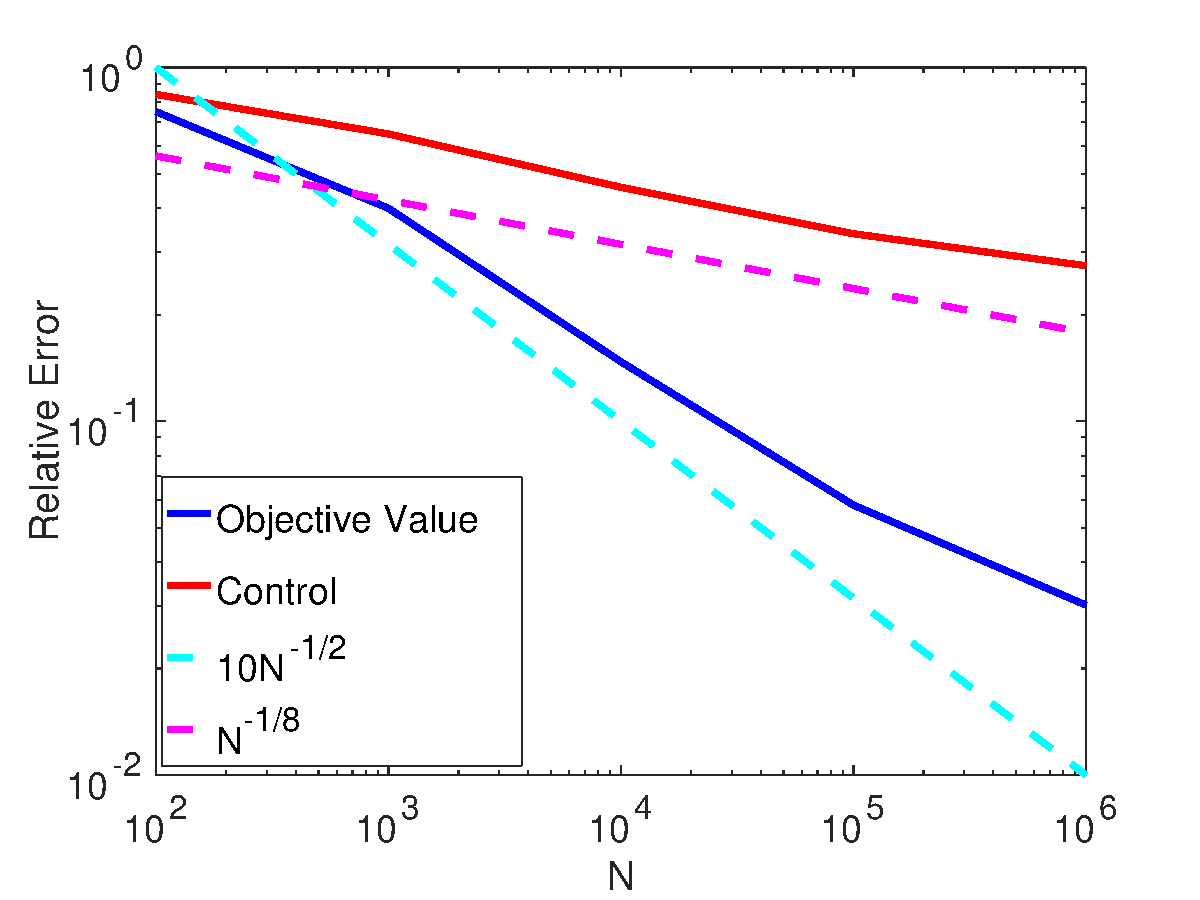
\includegraphics[width=0.4\textwidth,keepaspectratio]{Part I/figures/error.pdf}
\end{center}
\begin{exampleblock}{}\centering
\alert{Hundreds of millions} of \alert{PDE-solves} are needed to get an \textbf{accurate solution}.
\end{exampleblock}
\end{frame}


%%%%%%%%%%%%%%%%%%%%%%%%%%%%%%%%%%%%%%%%%%%%%%%%%

\begin{frame}\frametitle{}
\begin{center}\Large
Section 3\\
Algorithms for OUU\\
Part II: Empirical Approximation
\end{center}
\end{frame}

%%%%%%%%%%%%%%%%%%%%%%%%%%%%%%%%%%%%%%%%%%%%%%%%%

\subsection{Empirical Approximation: Pros, Cons, and Behavior in Practice} 

\begin{frame}\frametitle{Empirical Approximation}

\begin{exampleblock}{}
\begin{itemize}
\item
In the SA example, we expand the decision space by $t \in \mathbb R$ and consider
\[
 f(x) = \mathbb E_{\mathbb P_{\bm \xi}}[F(x,\cdot)] = \int_{\Xi} F(x,\xi) \, \mathrm{d} \mathbb P(\xi)
 \]
 \item  $F$ is \alert{nonsmooth} and convex. 
 \item $f$ involves a potentially high-dimensional integral. 
 \item We use quadrature everywhere in PDE-constrained optimization, why not here? 
 \item What are our options if $\mathrm{dim}\, \Xi \gg 1$?
 \end{itemize}
\end{exampleblock}
\visible<2->{
\begin{exampleblock}{}
\begin{itemize}
\item EA $=$ \textbf{E}mpirical \textbf{A}pproximations
\begin{itemize}
\item \textbf{M}onte \textbf{C}arlo (MC), 
\item \textbf{Q}uasi-\textbf{M}onte \textbf{C}arlo (QMC), Randomized QMC,
\item Deterministic quadrature approaches, e.g., \textbf{sparse grids}.
\end{itemize}
% \item Sample-\textbf{before}-you-go: Replace $f(x)$ by $\widehat{f}_{N}(x) = \int_{\Xi} F(x,\xi) \, \mathrm{d} \bbp_{N}(\xi) = \sum_{i=1}^{N} \pi_i F(x,\xi^i)$
\end{itemize}
\end{exampleblock}
}
\end{frame}

\begin{frame}\frametitle{Advantages}
\begin{exampleblock}{}
\begin{itemize}
% \item Recall again \eqref{eq:model_ra_op_prob_exp}, using an EA for the expectation leads to
% \begin{equation*}%\label{eq:model_ra_op_prob_exp_N}
% \aligned
% \mathrm{min}
% \left\{ 
% \widehat{f}_{N}(x) =
% \frac{1}{N} \sum_{i=1}^{N}
% \left[
% t + \frac{1}{2-2\beta}( \| S(z,\xi^i) - u_d \|^2_{L^2(D)} - 2t)_+ 
%   + \frac{\alpha}{2} \| z \|^2_{Z}
% \right] \text{ over } (z,t) \in \Zad \times \mathbb R 
% \right\}.
% \endaligned
% \end{equation*}
\item There have been enormous advances in nonlinear programming and numerical PDE-constrained optimization over the past several decades.
\visible<2->{
\item \textbf{Pro}: we may use a number of powerful optimization algorithms with convergence theory in a fully continuous setting.
}
\visible<3->{
\item \textbf{Pro}: For a fixed EA of the objective, the stopping criterion can be based on the residual of the first-order system.
}
\visible<4->{
\item \textbf{Pro}: Calculation of the $\omega$-dependent states, adjoint states, and Hessian vector products are parallelizable.
}
\end{itemize}
\end{exampleblock}
\end{frame}

\begin{frame}\frametitle{Parallelization in Smooth Linear Case}
\begin{exampleblock}{}
\begin{itemize}
% \item Keeping the spacial terms continuous, in an EA setting, e.g., Monte Carlo,  we would need:
\item Computing the reduced gradient $\nabla J(z)$ when using EA is largely parallelizable.
\item \textbf{$N$ states solves} (in parallel)
\[
\bm A(\xi^i) u = \bm B(\xi^i) z + f(\xi^i) \text{ in } H^{-1}(D)\quad i =1,\dots, N,
\]
\item \textbf{$N$ adjoint solves} (in parallel, serial with $i^{th}$ state $u^i$
\[
\bm A(\xi^i)^* \lambda = -J'_u(u(\xi^i),z) \text{ in } H^{-1}(D)\quad i =1,\dots, N,
\]
% which can also be done in parallel, but only when the $i^{th}$ state solve is available.
% \item \textbf{$N$ function evaluations}
% \[
% \phi'(G(x,\xi^i),\theta,r) \quad i =1,\dots, N
% \]
% Recall: $G(x,\xi) = \cJ(S(z,\xi)) - t$.
\item \textbf{$N$ ``matrix-vector''  products}
\[
\bm B ^*(\xi^i) \lambda(\xi^i) \quad i = 1,\dots, N.
\]
\item \textbf{$\approx N$ ``axpy's''} for the weighted sum : $\nabla \mathcal{J}(z) = -\frac{1}{N}\sum_{i=1}^N \bm B ^*(\xi^i) \lambda(\xi^i)$
\item \alert{Don't forget the Riesz maps/proper inner products}!
\end{itemize}
\end{exampleblock}
\end{frame}

\begin{frame}\frametitle{Parallelization in Smooth Linear Case}
\vspace{-1ex}
\begin{exampleblock}{}
\begin{itemize}
\item For each $\xi = \xi^{1},\dots,\xi^{N}$:
\item Define the Lagrangian:
$
\mathcal{L}(u,x,\lambda) = J(u,z) + \langle \bm A u - [\bm B z + f], \lambda \rangle_{U,U^*}
$
\visible<2->{
\item \textbf{$N$ state solves} $u(\xi)$: $\bm A(\xi) u(\xi) = \bm B(\xi) z + f(\xi)$
parallel for each $\xi$}
\visible<3->{
\item \textbf{$N$ adjoint solves} $\lambda(\xi)$: $\bm A^*(\xi) \lambda(\xi) = -J'_u(u(\xi),z)$
parallel for each $\xi$, serial in $u(\xi)$}
\visible<4->{
\item \textbf{$N$ state sensitivity solves} $w(\xi)$:
$
\bm A(\xi) w = \bm B(\xi) [v]_{z}.
$
parallel for each $\xi$
}
\visible<5->{
\item \textbf{$N$ adjoints sensitivity solves} $p(\xi)$:
\[
\bm A(\xi)^* p(\xi) = \mathcal{L}''_{uu}(u(\xi),z,\lambda(\xi))w - \mathcal{L}''_{uz}(u(\xi),z,\lambda(\xi))v.
\]
parallel for each $\xi$, serial in $u(\xi), \lambda(\xi)$ 
}
\visible<6->{
\item \textbf{$\xi$-dependent Hess-vec's}: \vspace{-1ex}
\[
H(z,\xi) v = \bm B(\xi)^*p(\xi) - \nabla_{zu} \mathcal{L}(u(\xi),z,\lambda(\xi))w + \nabla_{zz} \mathcal{L}(u(\xi),z,\lambda(\xi)) v.
\]\vspace{-4ex}
\item \textbf{aggregate, Riesz maps}.
}
\end{itemize}
\end{exampleblock}
\end{frame}



\begin{frame}\frametitle{Disadvantages (Opportunities!)}
\begin{exampleblock}{}
\begin{itemize}
\visible<1->{
\item \textbf{Con}: In contrast to SA-type methods, the convergence theory either works in the fully continuous (pre-EA) or the sample-based deterministic (post-EA) regime. 
}
\visible<2->{
\item \textbf{Con}: PDE-constrained optimization problems are large scale, the EA PDE-constrained problems can be significantly larger depending on $N$ even for low stochastic dimension. 
}
\visible<3->{
\item \textbf{Con}: Obtaining optimal sample sizes and rates of convergence (even a priori estimates) is challenging 
}
\visible<4->{
\item \textbf{Con}: The complexity of a single iterate can be significantly higher. For true scalability, need parallelization.
}
\visible<5->{
\item \textbf{Con}: Since the Hessian is only implicit, need to use iterative methods, which necessitate the development of preconditioners.
}
\visible<6->{
\item So if we're using second-order information and globalization strategies:\\  \centering How \alert{slow} could such an approach really be?
}
\end{itemize}
\end{exampleblock}
\end{frame}

\begin{frame}\frametitle{Is linear algebra \textit{\alert{really}} an issue?}
\begin{exampleblock}{}
\smaller
 The Robust Stochastic Mirror Descent method yielded the following:
 \begin{table}[]
\begin{tabular}{|c|c|c|c|c|c|c|}
\hline
iter  & time(s) & fval & abs-err $f$  & rel-err $f$  & abs-err $x_k$  &  rel-err $x_k$ \\
\hline
100         &  1.4     &   3.1274e-01 &   1.3403e-01 &    7.4999e-01 &   2.7098e+02  &  8.3928e-01\\
1000        & 14.7    & 2.5017e-01   & 7.1464e-02   &  3.9989e-01  &  2.0949e+02  &  6.4885e-01 \\
10000      & 152.0   &  2.0502e-01  &  2.6312e-02   &  1.4723e-01  &  1.4802e+02  &  4.5846e-01\\
100000    & 2054.2   &  1.8906e-01  &  1.0353e-02  &   5.7933e-02  &  1.0943e+02  &  3.3892e-01\\
{1000000}  & 104636.2  &   1.8411e-01 &   5.3994e-03 &    3.0213e-02 &   8.8822e+01 &   {2.7510e-01}\\
\hline
\end{tabular}
\end{table}

In contrast, using the PD-Risk (a second-order method) with Monte Carlo
\begin{table}[]
\begin{tabular}{|l|l|l|l|l|l|l|l|l|}%{lllllllll}
\hline

N   &      time(s)      &                 fval  &    nstate &   nadjoint  & nstatesens &  nadjointsens  & totalsolves \\
\hline
100     &    680.0    & 1.7924e-01    &   27500   &     7112    &    36554    &      36554    &    107720 \\
1000    &   2889.3   &  1.7871e-01   &    83000   &    30035    &   197168      &   197168    &    507371 \\
10000   &  23540.5   &  1.7871e-01  &    700000  &    268612    &  1594077    &    1594077     &  4156766 \\
%
 \hline
\end{tabular}
\end{table}
\end{exampleblock}
\end{frame}

%%%%%%%%%%%%%%%%%%%%%%%%%%%%%%%%%%%%%%%%%%%%%%%%%

\end{document}